\documentclass[../thesis/thesis.tex]{subfiles}
\renewcommand{\baselinestretch}{1.5}\selectfont
\graphicspath{{../figs/ch5-nlbmunc/}}

\begin{document}
	
\onlyinsubfile{\setcounter{chapter}{4}}

\begin{refsection}
\chapter[Prop. Meas. Unc. To Nonlinear Behavioural Models]{Propagating Measurement Uncertainty into Nonlinear Behavioural Models}
\section{Introduction}

The requirement of behavioural models for nonlinear microwave devices was introduced in Chapter 1 of this dissertation, where it was shown they can provide an intellectual-property-friendly ``black-box'' method to accurately predict device performance.

The core aim of a behavioural model is to fit mathematical functions to measurement data in order to reduce the amount of information stored within the extracted model (in contrast to a look-up table approach where the entire measurement dataset is indexed). This reduces both data storage requirements, making the model more portable, and also the computational requirements for accessing the model dataset when used in circuit simulators during design. Nonlinear behavioural models have developed over time and there are several different formulations in use today, of which the most common will be described in this Chapter. The reason there is no single ``best'' model is a question of application. Models which are most efficient and fit functions to more data dimensions may not be accurate for all device behaviours, whereas other models are more versatile but less data-efficient.

Before this project, no prior published work propagated a rigorous evaluation of measurement uncertainty through measurement data into an extracted nonlinear behavioural model. This information is of great use to both the modelling engineer, who can evaluate the sensitivities of their behavioural model to different sources of error in the measurement and extraction procedures, and the design engineer, who can quantify and compare the combined uncertainty in performance characteristics of circuits simulated using the extracted model. Both of these benefits will be presented in this Chapter.

%characterisation of amplifiers for digital pre-distortion \cite{Verspecht_2013,Kaur_2012}

\section{Nonlinear Behavioural Models}

We shall first introduce a generic frequency-domain model of the nonlinear device, illustrated in Figure X, which defines the various quantities required to understand the following behavioural models. The power waves $A$ and $B$ at port $n$ can be written as:

\begin{align}
	A_n &= \frac{V_n + I_n Z_n}{2\sqrt{\Re(Z_n)}} \\
	B_n &= \frac{V_n - I_n Z^*_n}{2\sqrt{\Re(Z_n)}},
\end{align}

where $V$ and $I$ are voltages and currents, respectively, and $Z$ is the port impedance - typically 50-Ohms.

\begin{figure}
	\centering
	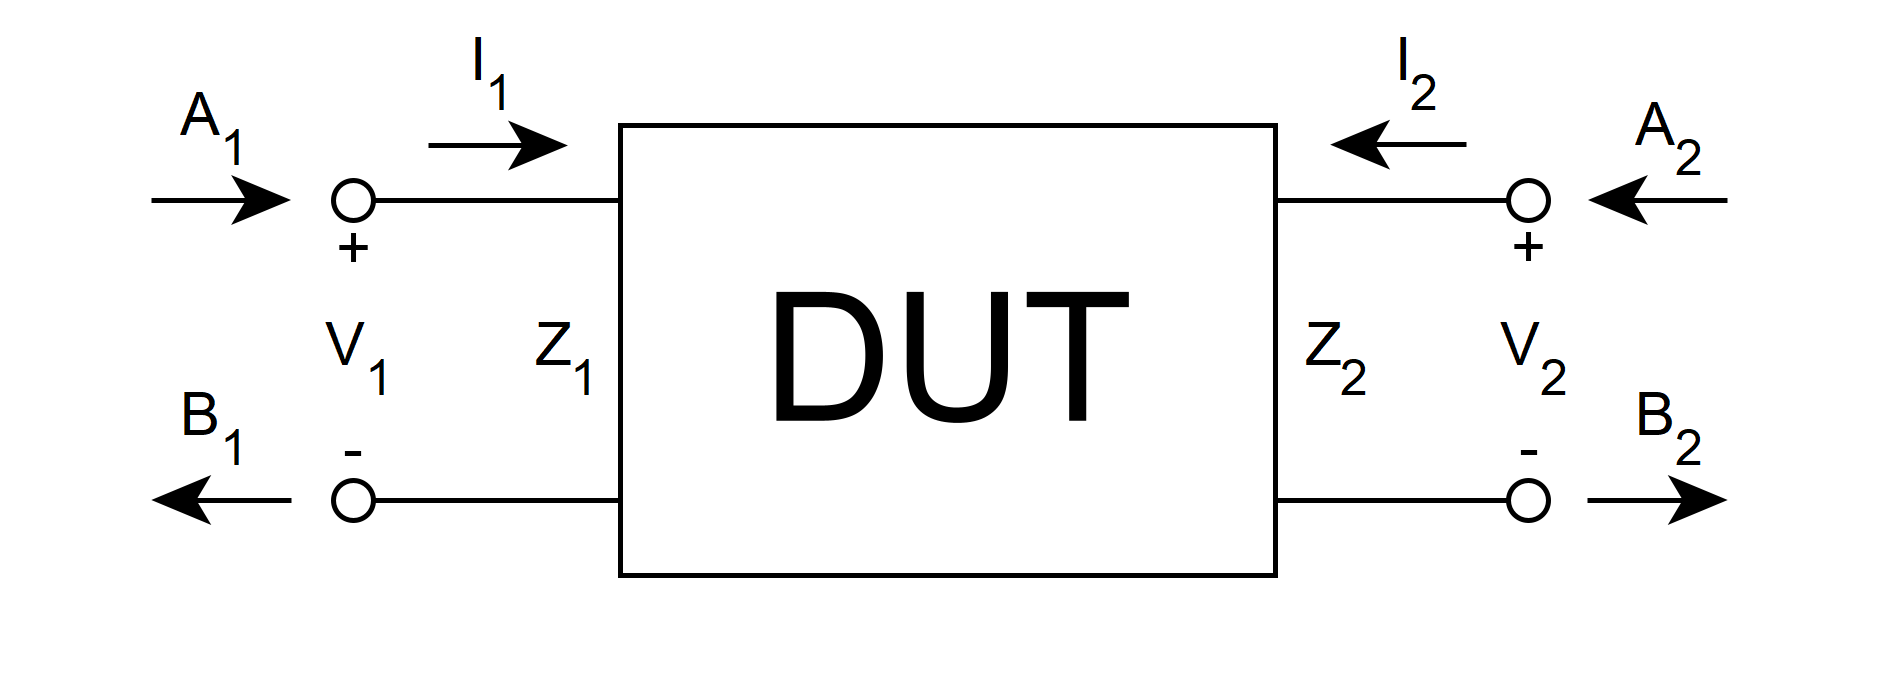
\includegraphics[width=0.65\textwidth]{dut}
	\caption[Device-under-test model representation.]{A representation of the different quantities described in nonlinear behavioural models, shown for a typical two-port device-under-test (DUT).}
	\label{ch5_fig_dut}
\end{figure}

\subsection{The Volterra ``VIOMAP'' Model}

One of the first examples of a nonlinear behavioural model for microwave amplifiers was the Volterra input-output map, or ``VIOMAP'' \cite{Verbeyst_1994}. This model was developed in the early nineties by Verbeyst and Vanden Bossche of the Hewlett Packard Network Measurement and Description Group (NMDG\footnote{now owned by National Instruments}) at Vrije University in Brussels. In an effort to find an S-parameter equivalent for nonlinear devices, VIOMAP replaces the parameters themselves with a sum of Volterra kernel components at each harmonic frequency\cite{Schetzen_2006, Moodi_2010}.

Although the VIOMAP model was shown to be cascadable \cite{Verbeyst_1994}, applicable across the Smith chart for efficient load-pull measurements \cite{Verbeyst_1995b}, and useful for characterising predistortion \cite{Verbeyst_1995}, it had two major shortcomings. Firstly, it could only be used to model weakly nonlinear devices. This issue was tackled by introducing orthogonal polynomials on which to base the Volterra kernel \cite{Verbeyst_1996}, although the choice of these polynomials was not clear to users and required a lot of computation, thus they were not widely adopted. Secondly, the measurement procedure was customised to suit different applications, which appeared to increase the barrier for entry to new users who could not confidently buy standard equipment to perform the measurements.

\subsection{Scattering Functions}

Scattering functions, originally termed describing functions from their nonlinear analysis origin, were introduced by Verspecht and reduced the computational overhead for modelling strong nonlinearities when compared to the VIOMAP model \cite{Verspecht_1996}. They are expressed as a function mapping $N$ complex numbers representing the input signal $A$ into the $k^{\textrm{th}}$ spectral component of the output signal $B$:

\begin{equation}
	B_{k} = F_k(A_1, A_2, \dots, A_N),
	\label{ch5_eqn_scatfunc}
\end{equation}

where $F_k$ is the scattering function for $k$. The VIOMAP model can be shown to be a subset of the scattering function approach, where the functions are constrained to a limited set of polynomials.

It should be mentioned here that all models described in this section require the device to be time-invariant, meaning that a time delay (or phase shift) in the input signal causes an equivalent time delay (or phase shift) in the output signal. This is typically the case for amplifiers, but more integrated communications components which include, for example, internal oscillators, cannot be modelled using the approaches described in this chapter.

Similar to the VIOMAP model, scattering functions are also complicated to apply and were not popular as a nonlinear modelling paradigm.

\subsection{Hot S-parameters}

Hot S-parameters were developed as a nonlinear behavioural model to extend S-parameters and allow stability and distortion characterisation of amplifiers \cite{Verspecht_2002, Verspecht_2005}. The model has several variations depending on the behaviour of interest, and there also exists an enhanced hot S-parameter model which incorporates additional information (in anticipation of the polyharmonic distortion model and the X-parameter model derived from it, which is described later).

Fundamentally, the hot S-parameter model, when used to characterise the distortion of amplifiers, provides a set of S-parameter measurements which are indexed against both frequency $f$ (like standard S-parameters) and also the amplitude of the incident tone $|a_1|$:

\begin{equation}
	\begin{bmatrix}
		B_1(f) \\ 
		B_2(f) 
	\end{bmatrix}
	= 
	\begin{bmatrix}
		hotS_{11}(f, |A_1|) & hotS_{12}(f, |A_1|) \\
		hotS_{21}(f, |A_1|) & hotS_{22}(f, |A_1|)
	\end{bmatrix}
	\begin{bmatrix}
	A_1(f) \\ 
	A_2(f) 
	\end{bmatrix}
\end{equation}

The enhanced version of the model includes two additional parameters which describe more completely the nonlinear output matching characteristic ($hotS_{22}$):

\begin{equation}
	\begin{bmatrix}
		B_1(f) \\ 
		B_2(f) 
	\end{bmatrix}
	= 
	\begin{bmatrix}
		hotS_{11}(f, |A_1|) & hotS_{12}(f, |A_1|) \\
		hotS_{21}(f, |A_1|) & hotS_{22}(f, |A_1|)
	\end{bmatrix}
	\begin{bmatrix}
		A_1(f) \\ 
		A_2(f) 
	\end{bmatrix}
	+
	\begin{bmatrix}
		T_{12}(f, |A_1|) \\ 
		T_{22}(f, |A_1|) 
	\end{bmatrix}
	e^{j\phi(A_1(f))}A_2^*(f)
	\label{ch5_eqn_hotsp}
\end{equation}

where $e^{j\phi(a_1(f))}$ normalises the phase of $a_2$ relative to $a_1$, $a_2^*$ is the conjugate of $a_2$ and $T_{ij}$ are the two new parameters in the enhanced model.

For an amplifier operating in the nonlinear regime, both the magnitude and phase of reflections at the output, due to matching, can have a significant impact on the device performance \cite[Figure 12.13]{Cripps_2006}. Figure \ref{ch5_fig_hots22} illustrates versions of the hot S-parameter model with different $hotS_{22}$ definitions.

The amplifier stability form of hot S-parameters will not be discussed here, but an overview is available in \cite{Verspecht_2005}.

\begin{figure}
	\centering
	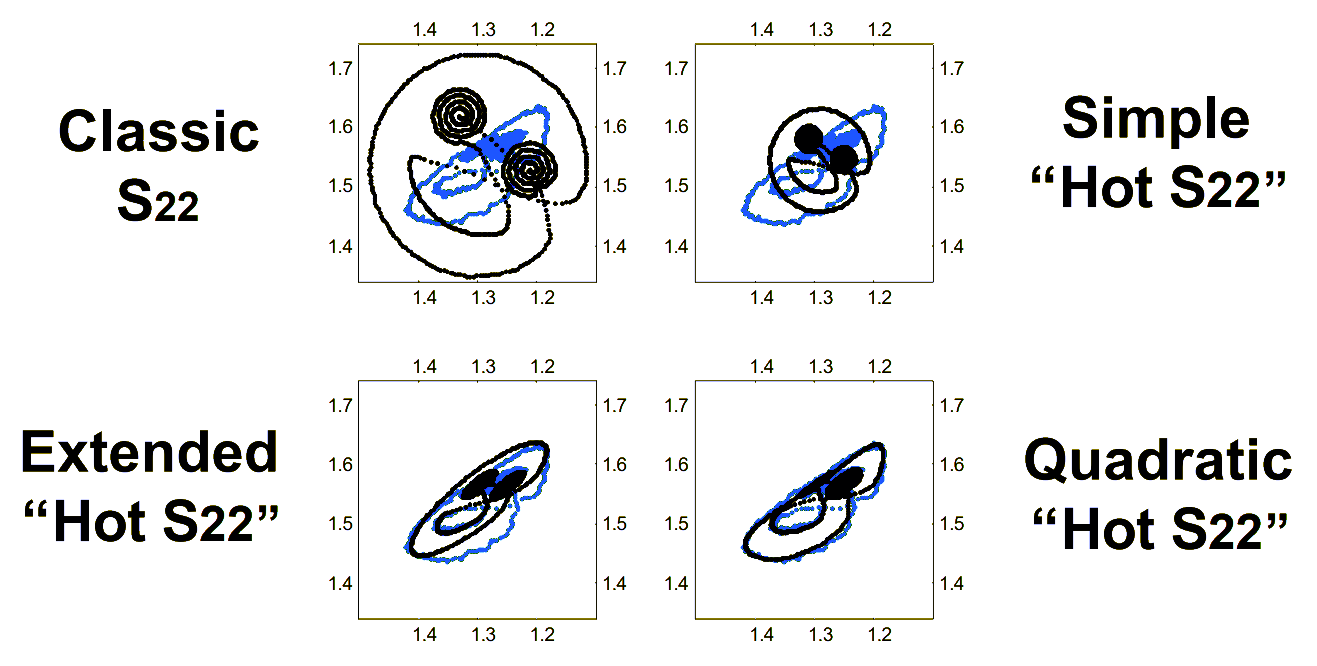
\includegraphics[width=\linewidth]{hots22_recoloured}
	\caption[Performance of hot S-parameter models with different $hotS22$ definitions.]{Performance of hot S-parameter models with different $hotS22$ definitions, showing in polar form the measured (blue) and predicted (black) $b_2$ wave for a modulated large-signal $a_1$ wave, with values in Volts. Classic $S_{22}$ means no dependence of $S_{22}$ on $|a_1|$, simple ``Hot S22'' means a linear dependence of $S_{22}$ on $|a_1|$, extended ``Hot S22'' includes dependence of $S_{22}$ on $|a_1|$ and $a_2$, and quadratic ``Hot S22'' includes a second order dependence of $S_{22}$ on $a_2$ \cite{Verspecht_2002}.}
	\label{ch5_fig_hots22}
\end{figure}

\subsection{X-Parameters}

X-parameters \cite{Root_2013}, from Keysight, are the commercial realisation of the poly-harmonic distortion model \cite{Verspecht_2006}, which itself is an application of scattering functions with particular constraints. The most significant constraint is that any output of device which the model is applied to behaves linearly with respect to incident tones at harmonics of the fundamental, which is illustrated in Figure \ref{ch5_fig_superposition}. 

\begin{figure}
	\centering
	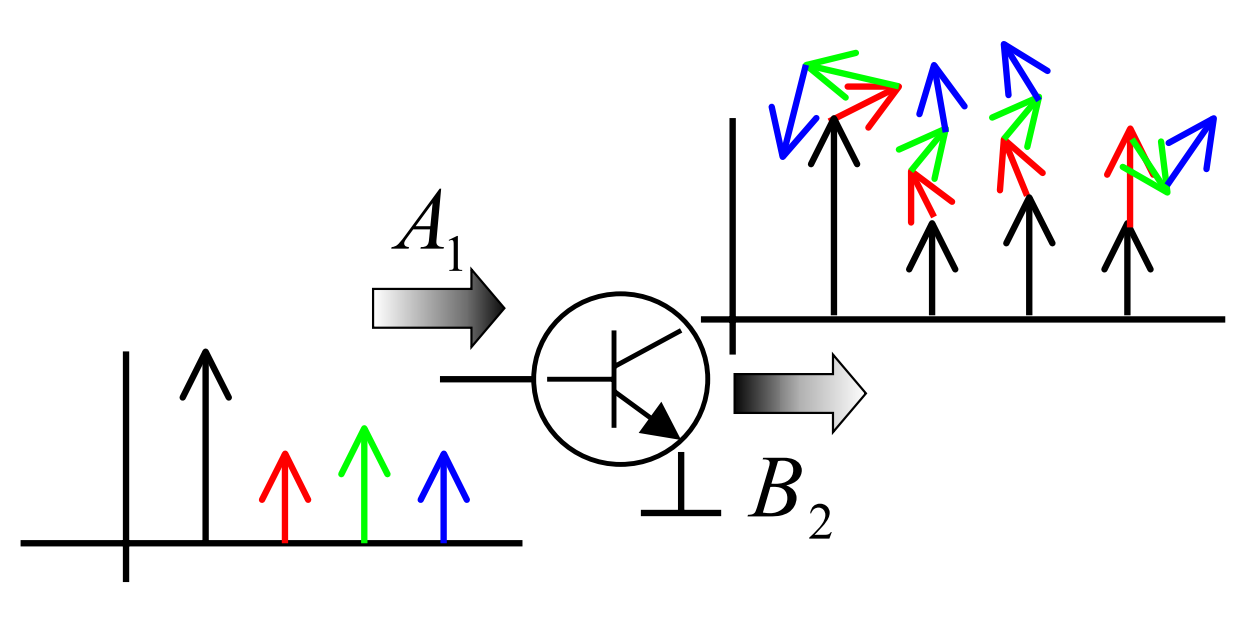
\includegraphics[width=0.65\textwidth]{superposition}
	\caption[The harmonic superposition principle.]{The harmonic superposition principle. If the input at port one ($A_1$) contains several small-signal harmonics, the output at port two ($B_2$) will comprise of the large-signal response plus the sum of responses due to each small-signal input harmonic, at each frequency \cite{Verspecht_2006}. The plots show complex phasors of increasing harmonic index along the horizontal axis, where the colour of the output phasors relate to the contribution from the respective input phasor.}
	\label{ch5_fig_superposition}
\end{figure}

The X-parameter formulation can be developed from the scattering function origin. Firstly, the output $B_{p, k}$, at port $p$ and harmonic $k$, is defined as:

\begin{equation}
	B_{p, k} = \sum_{q,l}S_{p, k;q, l}(|A_{1,1}|)P^{k-l}A_{q, l} + 
	\sum_{q,l}T_{p, k;q, l}(|A_{1,1}|)P^{k+l}A_{q, l}^*,
\end{equation}

where $A_{q,l}$ is the input at port $q$ and harmonic index $l$, and $P$ is a phase normalisation coefficient such that $P=e^{j\phi(A_{1,1})}$, similar to (\ref{ch5_eqn_hotsp}). This equation contains two scattering functions which are sensitive to the large-signal input at the fundamental, $A_1,1$. The second function, $T_{p, k;q, l}$, is identical to $S_{p, k;q, l}$ except that it is a coefficient of the conjugate of the input wave, $A_{q, l}^*$. As with the enhanced Hot S-parameters, this is a more generalised way to incorporate the sensitivity of the model to the phase of input signals at harmonics on any port. Mathematically, the requirement of these two functions is a result of the non-analyticity of the complex-valued scattering functions. It is possible to instead define the functions in terms of real and imaginary components, but the normal and conjugate definition is standard for X-parameters and so will be taken forward here.

Because the phase is normalised with respect to that of $A_{1, 1}$, we can also define $T_{p,k;1,1}=0$ as the entire device response for this port and harmonic combination will be captured in $S_{p,k;1,1}$, which also represents the response to the large-signal input at port one at the fundamental tone. If we assume that the harmonic superposition principle is valid for our model, we can then simplify it by extracting the large-signal response as a separate term and treat the remaining functions as linear, with the restriction that they do not apply when $q, l = 1, 1$. A good overview of this linearisation process of scattering functions is provided in \cite{Verspecht_2005b}.

We can now write our model as:

\begin{equation}
\begin{split}
B_{p, k}=X^\textrm{F}_{p, k}(|A_{1, 1}|)P^k+\sum_{q, l\ne(1,1)}[X^\textrm{S}_{p, k;q, l}(|A_{1, 1}|)A_{q, l}P^{k-l}\\+X^\textrm{T}_{p, k;q, l}(|A_{1, 1}|)A^*_{q, l}P^{k+l}],
\end{split}
\label{ch5_eqn_xps}
\end{equation}
where $X^\textrm{F}$ (the large-signal term), $X^\textrm{S}$ and $X^\textrm{T}$ (the small-signal terms) are called X-parameters.

Two informative comparisons between the performance of scattering functions and X-parameters in modelling nonlinear device behaviour can be found in \cite{Sun_2010,Widemann_2015}.

The X-parameter model is heavily marketed by Keysight to be a complete solution for modelling nonlinear device behaviour. Additions to the model include mixer characterisation using multi-tone stimuli \cite{Xie_2012}, the inclusion of memory effects \cite{Verspecht_2009}, the prediction of load-pull performance from a single X-parameter measurement at 50-Ohms \cite{Root_2017}, and recently the inclusion of electro-thermal effects \cite{Gillespie_2018}. The X-parameters themselves are closely related to elements of the Jacobian matrix used within harmonic balance simulations. This feature means that X-parameters can be extracted in a straightforward way from circuit simulations, and existing X-parameter models based on measurements can be included in simulations. At least two circuit simulators support X-parameter models at the time of writing, including Keysight Advanced Design System (ADS) \cite{ADS} and National Instruments AWR Microwave Office \cite{AWR}.

\subsection{The Cardiff Model}

Although X-parameters are sufficient to characterise the nonlinear behaviour of many amplifiers, the standard model\footnote{It is possible to extend the X-parameter model to include higher order mixing products, however this is not supported by commercial measurement or simulation solutions.} only includes third-order mixing products (via the $P^{(.)}$ terms in (\ref{ch5_eqn_xps})). While the harmonic superposition principle holds, which is the case for weak-to-moderate nonlinear devices with well-matched ports, this is not always true for strongly nonlinear devices such as unpackaged transistors, amplifiers driven in class F modes, or devices with port impedances far from 50-Ohms. In order to avoid this X-parameters can be extracted as a function of both $|A_{1,1}|$ and $A_{2,1}$, but this can increase the model size significantly, especially for load-pull applications with phase and magnitude sweeps of $A_{2,1}$ \cite{Gunyan_2009}. An alternative approach,  The Cardiff model, named after it's origin at Cardiff University, UK, incorporates $n^{\textrm{th}}$-order mixing products (typically truncated to seventh-order terms) and reduces the model dependence for fundamental load-pull to $|A_{1,1}|$ and $|A_{2,1}|$ only \cite{Woodington_2008,Qi_2009}.

The formulation of the Cardiff model is represented differently to that of X-parameters, however, they are a natural extension of that model and are equivalent when used with third-order mixing products. The measurement and extraction process is usually performed with a sampler-based NVNA featuring a real-time sampling oscilloscope and consists of a load-pull measurement \cite{Woodington_2010}.

For this project, X-parameters were chosen as the nonlinear behavioural model for which to focus on developing an uncertainty propagation, due to their current popularity. The framework which has been developed can be extended to include other models, but does not currently support them. Therefore, the Cardiff model will not be discussed in any greater detail here.

\begin{figure}
	\centering
	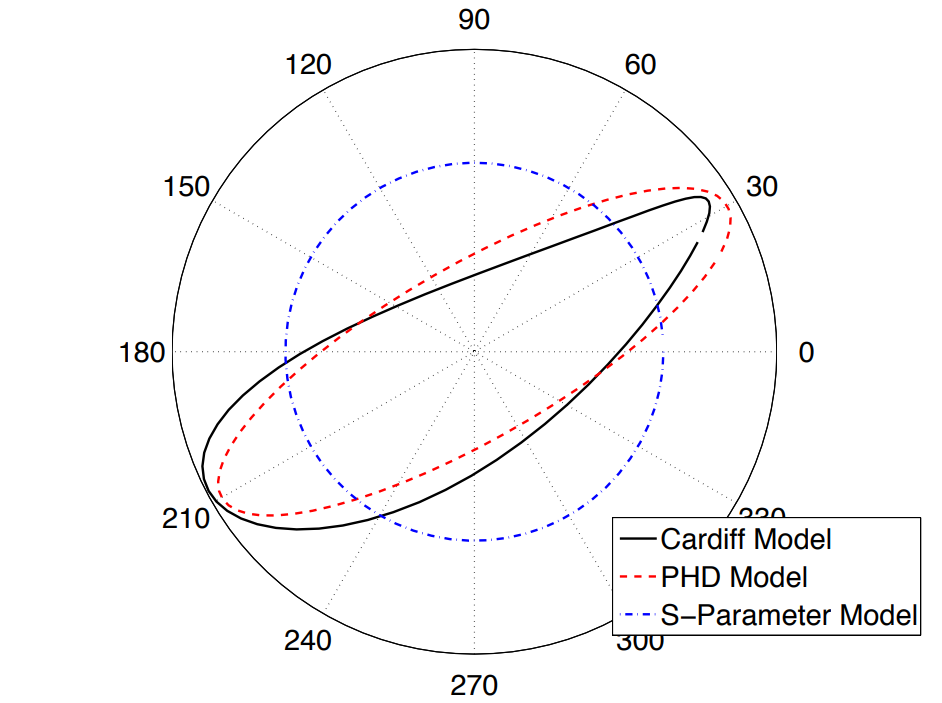
\includegraphics[width=0.65\textwidth]{phasedep}
	\caption[Relationship of device output against input wave phase for different nonlinear behavioural models.]{The relationship of device output $b_{p,k}$ against varying input wave phase $\angle a_{q,l}$ ($q, l \ne 1, 1$) for different nonlinear behavioural models, showing the effect that higher order mixing products have on the accuracy of the model \cite{Bespalko_2016}.}
	\label{ch5_fig_phasedep}
\end{figure}

\section{X-Parameter Extraction Procedure}

X-parameters can be extracted from either measured or simulated data. A least-squares estimation can be used for both cases, however it is often more efficient to extract X-parameters directly from harmonic balance internal variables when simulating data. This section will describe the process involved for the least squares estimation of X-parameters from measured data, and two implementations developed during this project.

\subsection{Method}

To perform device measurements from which X-parameters can be extracted, an NVNA setup as shown in Chapter 2 must be prepared, with the additional requirement of a second signal source which can be applied at either of two ports. All measurements taken during this project used the following Keysight equipment: an N5247A PNA-X NVNA, N1913A EPM Series Power Meter and two U9391G Comb Generators as phase references. Variables used in this section are in reference to (\ref{ch5_eqn_xps}).

The large-signal X-parameter, $X_\textrm{F}$, is simple to measure as it captures to the response of the device to a single large-signal drive tone at the fundamental frequency on port one ($A_{1,1}$). It is indexed against $|A_{1,1}|$, so this power is swept and measurements at each port $p$ and harmonic $k$ are made. The drive tone amplitude $|A_{1,1}|$ is said to define a large-signal operating point (LSOP) against which all of the X-parameters are indexed.

The small-signal X-parameters, $X_\textrm{S}$ and $X_\textrm{T}$, model the interactions between small-signals incident to the device and $A_{1,1}$. To capture this behaviour, measurements are made with a second tone (``extraction'' or ``tickler'' tone) applied to each port and harmonic in turn. If we ignore the conjugate term X-parameter $X_\textrm{T}$ (which is similar to the simple ``Hot S22'' model in Figure \ref{ch5_fig_hots22}), these measurements are all that is required to extract X-parameters. This equates to $N + N \times Q \times L$ stimulus conditions, where $N$ is the number of LSOPs, $Q$ is the number of ports and $L$ is the number of harmonics. For each stimulus condition, the NVNA measures the device output on all ports at each harmonic. A diagram of the NVNA setup required for these measurements is shown in Figure \ref{ch5_fig_nvna}.

\begin{figure}
	\centering
	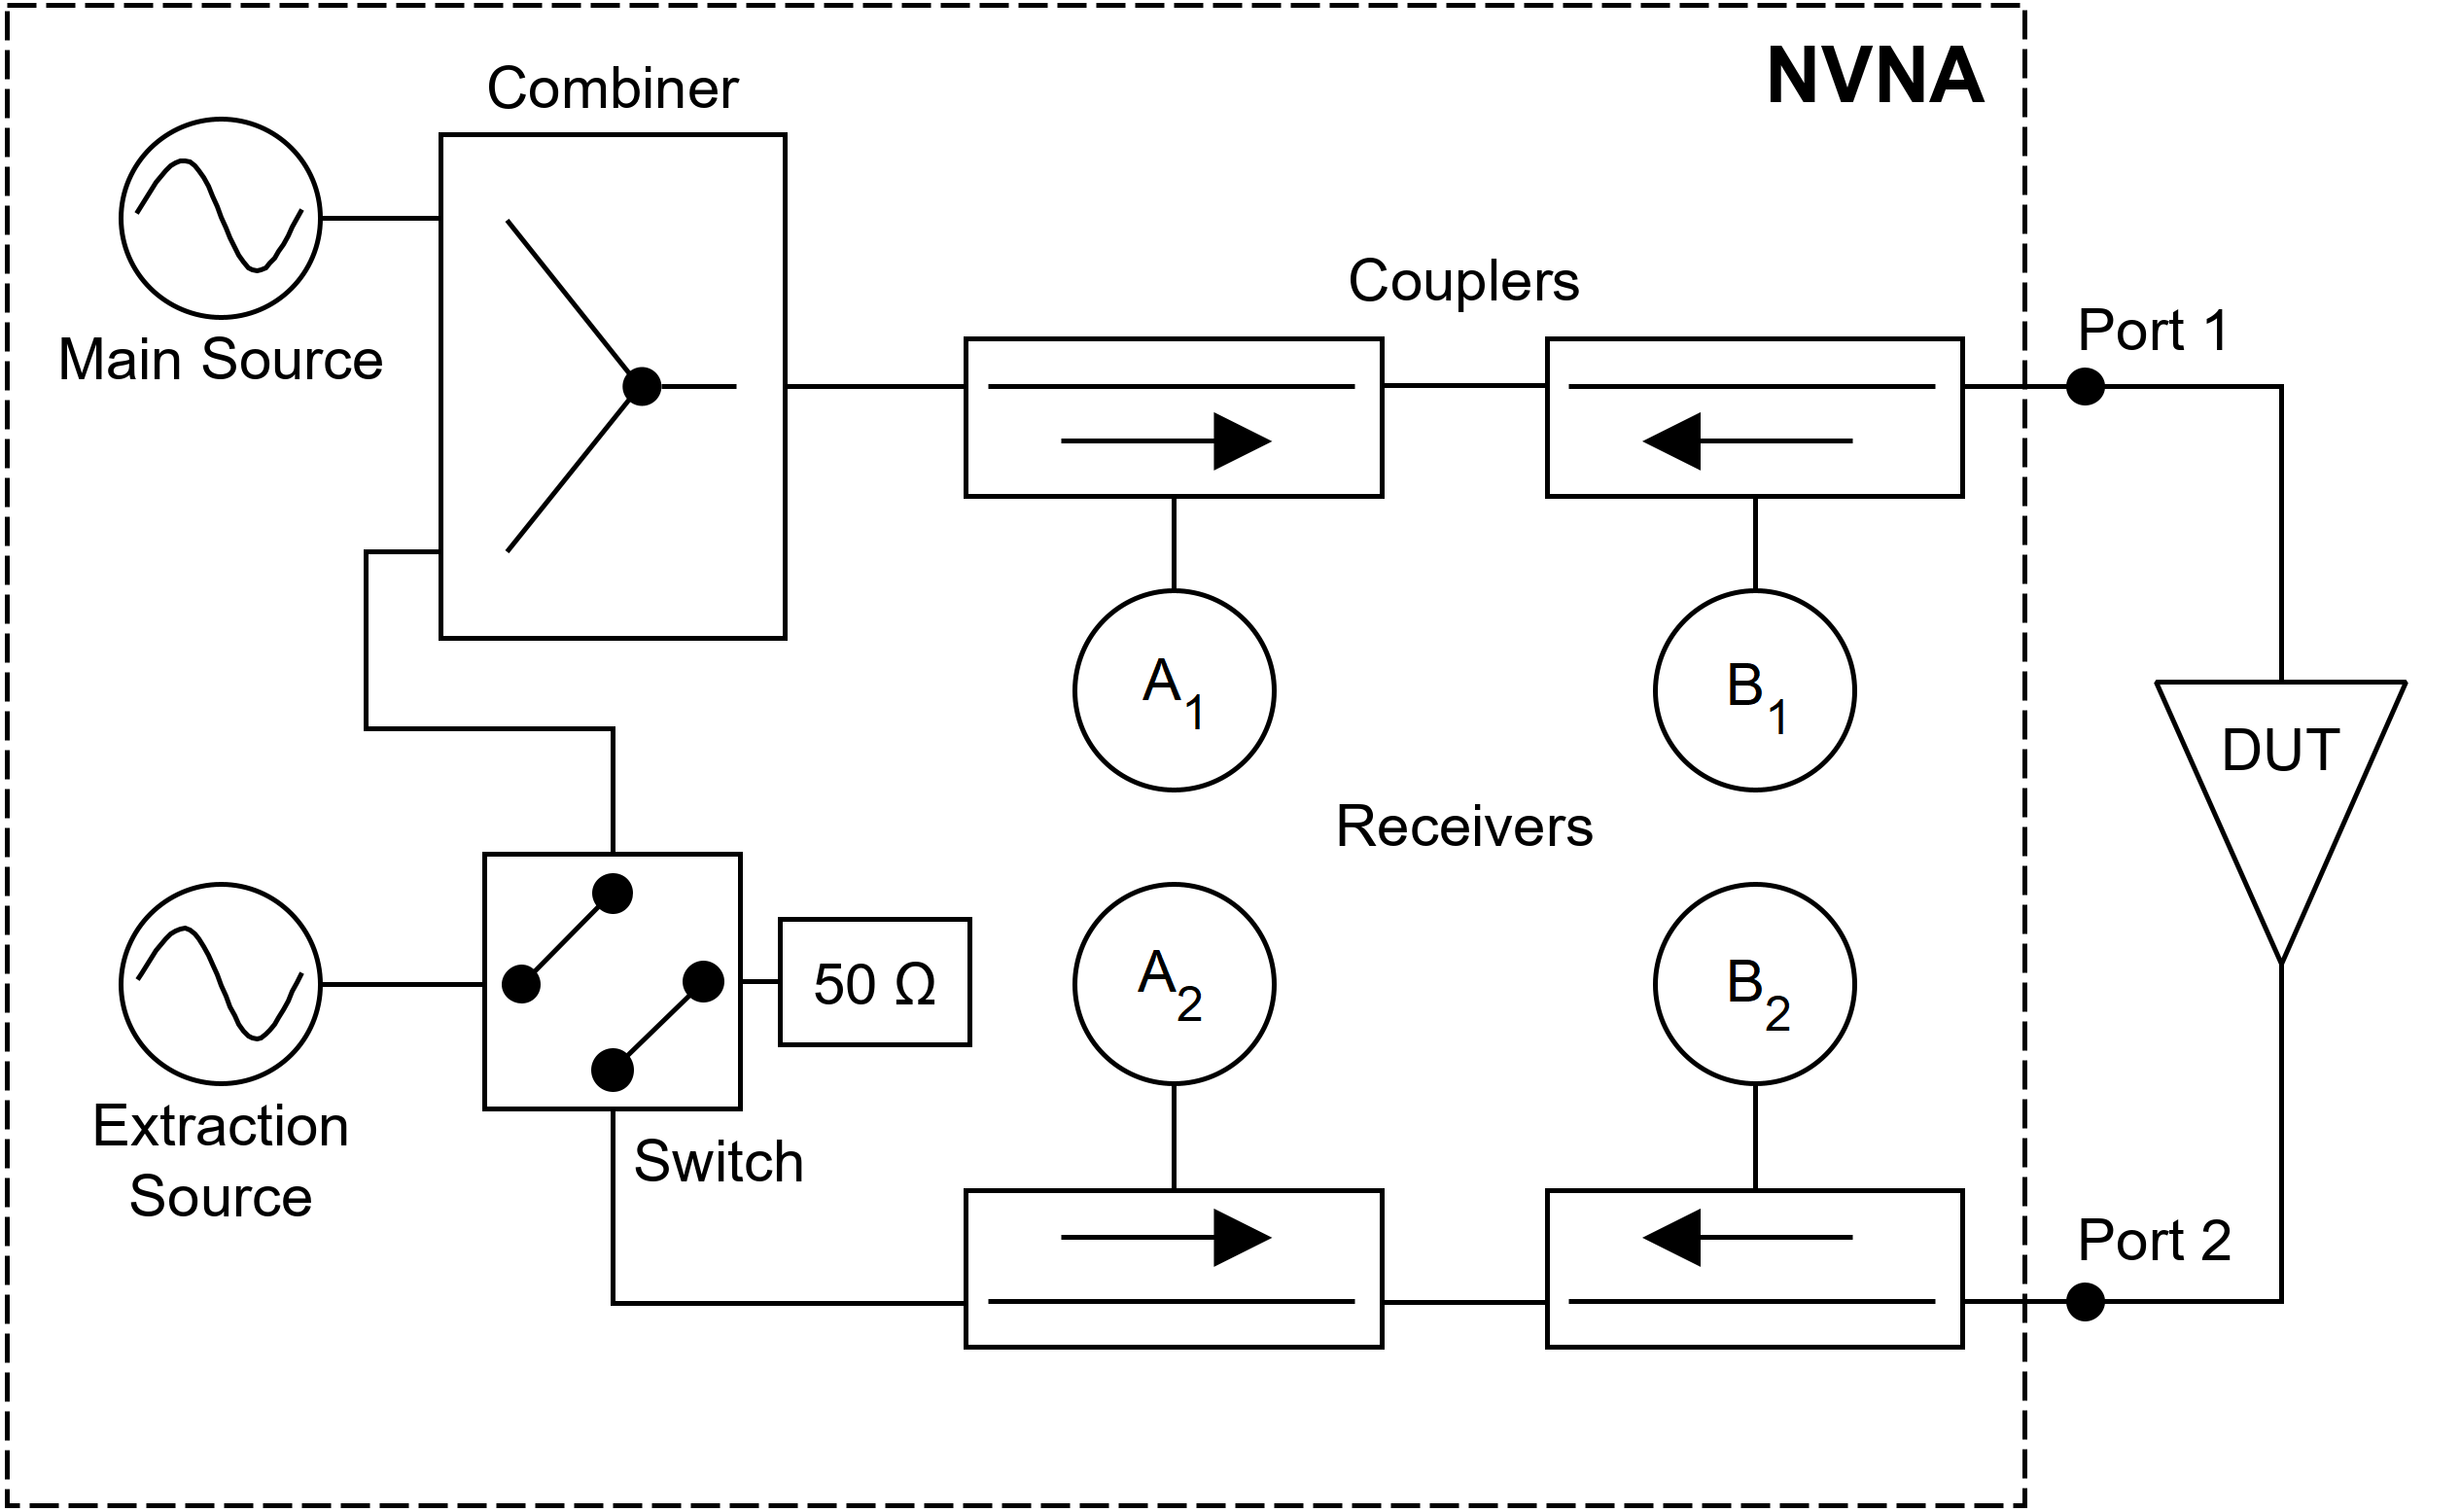
\includegraphics[width=0.8\textwidth]{nvna}
	\caption[NVNA setup required for X-parameter measurements.]{The NVNA setup required for X-parameter measurements. The switch terminates the unused port to a 50-Ohm load. The phase reference is connected to a spare receiver but not shown.}
	\label{ch5_fig_nvna}
\end{figure}

However, to extract the full X-parameter model we must make additional measurements to characterise the phase-dependence of the mixing products between the extraction tones and the LSOP. This is the behaviour captured by the $X_\textrm{T}$ parameters. Two measurement methods were developed to perform this task: offset-frequency and offset-phase. The offset-frequency method is not supported by the current version of the PNA-X firmware and appears to have fallen out of use, so the offset phase method alone will be explained. Further information can be found in \cite{Root_2013}.

Instead of a single extraction tone applied at each port and harmonic, a second measurement must be performed at an orthogonal phase ($\theta+90^{\circ}$) to the initial extraction tone. An illustration of these measurements using phasors is given in Figure \ref{ch5_fig_extract}. After subtracting the large-signal only measurement from these two new measurements, we obtain two small-signal contributions which can be used to solve the following equations:

\begin{align}
	B^{SS1}_{p,k} &= X^\textrm{S}_{p,k,q,l}A^{SS1}_{q,l} + X^\textrm{T}_{p,k,q,l}(A^{SS1}_{q,l})^*, \\
	B^{SS2}_{p,k} &= X^\textrm{S}_{p,k,q,l}A^{SS2}_{q,l} + X^\textrm{T}_{p,k,q,l}(A^{SS2}_{q,l})^*.
\end{align}

To improve noise errors it is advisable to make more than two measurements of different extraction tone phases (typically four) and solve for $X_\textrm{S}$ and $X_\textrm{T}$ using a least-squares estimation. The extraction tone amplitude should be as low as possible to ensure that the device is responding linearly to the added tone (it is effectively performing a perturbation analysis described in Chapter 3), and Keysight suggests that it should be 16 dB below the largest LSOP signal. The extraction process can in fact be simplified further by using a matrix least-squares arrangement to solve for the entire X-parameter model, which removes the need to subtract the large-signal response from all the extraction tone measurements. If we define a matrix $\bm{A}$ such that each row contains the NVNA measurements for a single extraction tone stimulus (from 1 to $QL$, with 0 being no extraction tone):

\begin{figure}
	\centering
	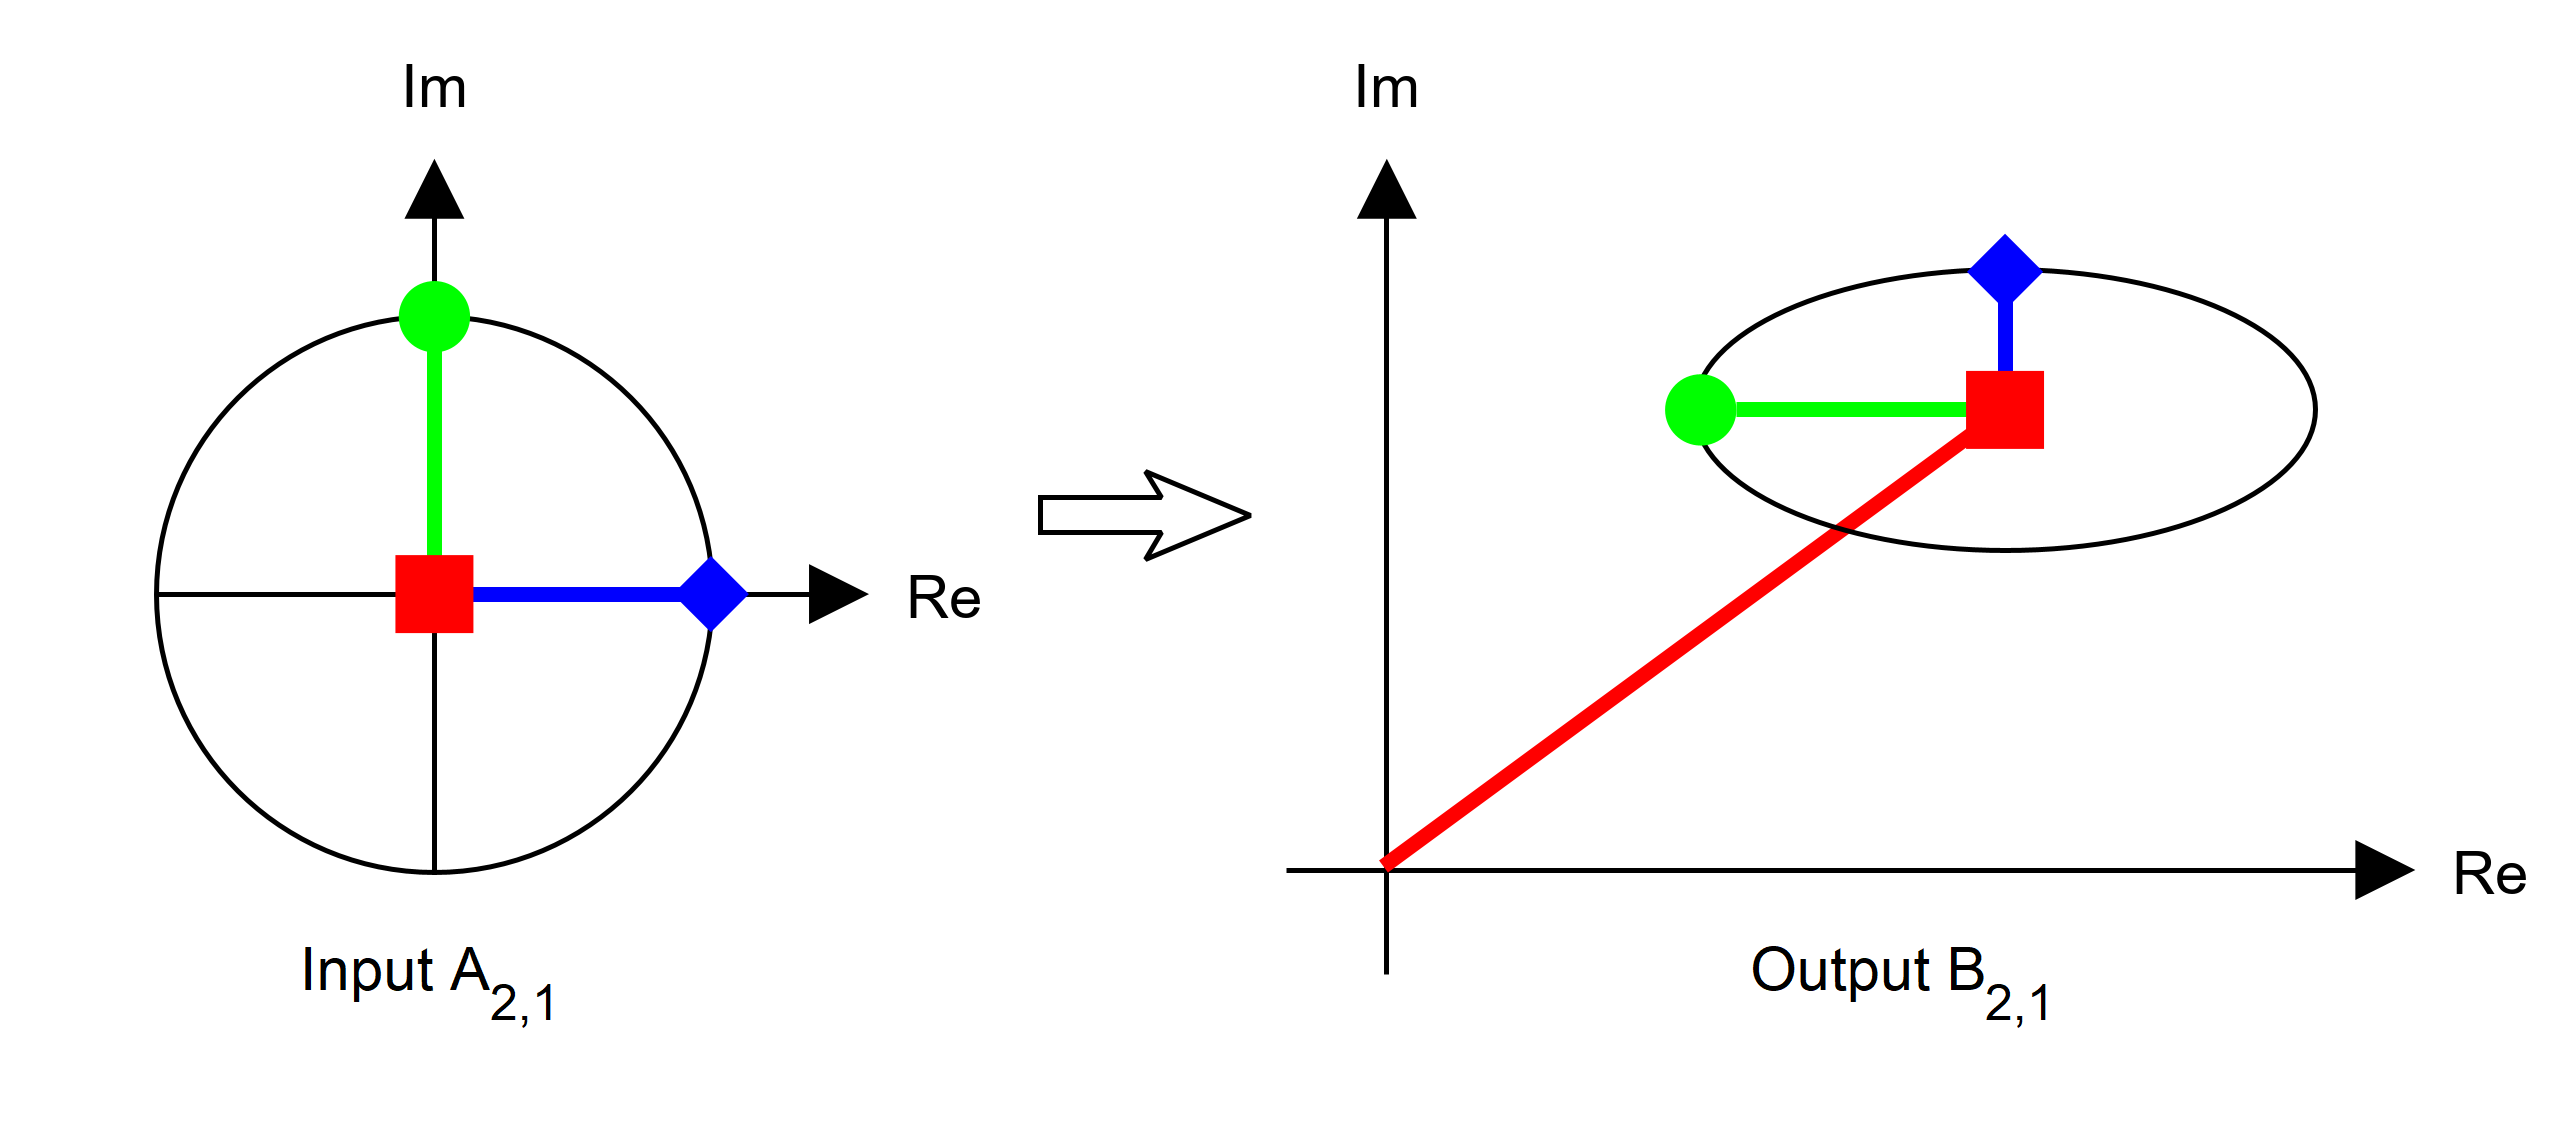
\includegraphics[width=\textwidth]{extract}
	\caption[Offset-phase X-parameter extraction procedure.]{An example of the offset-phase method for measuring device response for X-parameter extraction. The red square stimulus is with no extraction tone, and the blue diamond and green circle stimuli are with extraction tones applied at $0^{\circ}$ and $90^{\circ}$, respectively. Although $A_{2,1}$ and $B_{2,1}$ are specified, this effect occurs for all tones other than the fundamental on port one \cite{Verspecht_2006}.}
	\label{ch5_fig_extract}
\end{figure}

\begin{equation}
	\bm{A} =
	\begin{bmatrix}
		1 & A_{(1,1)_0} & A_{(2,1)_0} & A^*_{(2,1)_0} & A_{(1,2)_0} & A^*_{(1,2)_0} & A_{(2,2)_0} & A^*_{(2,2)_0} & \dots \\
		1 & A_{(1,1)_1} - A_{(1,1)_0} & A_{(2,1)_1} & A^*_{(2,1)_1} & A_{(1,2)_1} & A^*_{(1,2)_1} & A_{(2,2)_1} & A^*_{(2,2)_1} & \dots \\
		1 & A_{(1,1)_2} - A_{(1,1)_0} & A_{(2,1)_2} & A^*_{(2,1)_2} & A_{(1,2)_2} & A^*_{(1,2)_2} & A_{(2,2)_2} & A^*_{(2,2)_2} & \dots \\
		\vdots & \vdots & \vdots & \vdots & \vdots & \vdots & \vdots & \vdots & \dots \\
		1 & A_{(1,1)_{QL}} - A_{(1,1)_0} & A_{(2,1)_{QL}} & A^*_{(2,1)_{QL}} & A_{(1,2)_{QL}} & A^*_{(1,2)_{QL}} & A_{(2,2)_{QL}} & A^*_{(2,2)_{QL}} & \dots \\
	\end{bmatrix}
\end{equation}

and a vector $\bm{b}_{p,k}$ of length $QL$ is defined to contain the respective measurements of a single output wave $b_{p,k}$:

\begin{equation}
	\bm{b}_{p,k} =
	\begin{bmatrix}
		B_{(p,k)_0} \\
		B_{(p,k)_1} \\
		\vdots \\
		B_{(p,k)_{QL}} \\
	\end{bmatrix},
\end{equation}

then the X-parameters can be solved for using the following least-squares estimation:

\begin{equation}
	\bm{\hat{X}}_{p,k} = (\bm{A}^\top \bm{A})^{-1}\bm{A}^\top \bm{b}_{p,k}
\end{equation}

with the vector $\bm{\hat{X}}_{p,k}$ containing X-parameters:

\begin{equation}
	\bm{\hat{X}}_{p,k} = 
	\begin{bmatrix}
		X^\textrm{F}_{p,k} \\
		X^\textrm{S}_{p,k, 1, 1} \\
		X^\textrm{S}_{p,k, 2, 1} \\
		X^\textrm{T}_{p,k, 2, 1} \\
		X^\textrm{S}_{p,k, 1, 2} \\
		X^\textrm{T}_{p,k, 1, 2} \\
		X^\textrm{S}_{p,k, 2, 2} \\
		X^\textrm{T}_{p,k, 2, 2} \\
		\vdots \\
	\end{bmatrix}.
\end{equation}

The parameter $X^\textrm{T}_{p,k, 1, 1}$ will always equal zero for conventional measured X-parameters because the phase normalisation (time shift) which occurs during measurement means that any extraction tone applied to port one at the fundamental will always have the same phase value. Therefore, effectively $X^\textrm{S}_{p,k, 1, 1}$ from measured X-parameters equals $X^\textrm{S}_{p,k, 1, 1} + X^\textrm{T}_{p,k, 1, 1}$ from simulated X-parameters extracted from harmonic balance simulations, where this stage of phase normalisation is not performed. For the latter, the response is correctly separated between the two X-parameters, which means that this phase-dependence information is captured correctly. 

\subsection{Implementation}

The PNA-X NVNA contains a specific firmware for nonlinear measurements and a software option to allow X-parameter measurements to be performed and the model extracted on the NVNA itself. This is adequate for typical user requirements and the processing time is relatively fast (up to a few seconds) compared with the duration of measurements (hours for dense LSOP sweeps with several harmonics). However, to propagate uncertainty into X-parameters using this extraction method with numerical techniques supported by the MUF is very time-consuming, and practically restricts the number of Monte Carlo samples which can be used to perform the uncertainty propagation. For the experiments performed in this project, over 300 sources of error are included from the nonlinear measurements. This means that at least 300 X-parameter extractions must be computed for the sequential perturbation and sensitivity analysis alone. For these reasons, only 1000 Monte Carlo samples were used, which was deemed appropriate by resampling using bootstrap methods \cite{Chernick_2008}.

Once X-parameter measurements have been performed and the parameters themselves automatically extracted, it is possible to save not only the X-parameters (as a ``.xnp'' file), but also the X-parameter measurements (as a ``.xmeas'' file), which contain tables of power wave measurements relating to all sweeps, including those of extraction tone stimuli. This file is then loaded into the MUF as a DUT measurement to be propagated through the calibration measurement model, as described in Chapter 3. The addition of X-parameter measurement file support to the MUF was included as part of this project, with support from the developers. During this work, several further additions and improvements were made to the software, including file access changes which reduced the processing time of all MUF uncertainty evaluations by a factor of at least 100. Once the X-parameter measurements have been perturbed as part of the uncertainty propagation, they are then sent back to the NVNA for X-parameter extraction, which is detailed in the following section.

The NVNA does not need to be calibrated before the X-parameter measurements are performed because the power waves will be instead corrected during the MUF calibration step. However, it does not affect the result if a preliminary calibration is performed, and it can be useful to verify that the calibration standards are in good order and the DUT is behaving as expected.

To address the issue of slow extraction for large numbers of perturbed measurements, an alternative  X-parameter extractor was implemented from scratch as a MUF post-processor (measurement model). This would allow the samples to be run on more powerful hardware than the NVNA onboard computer, and even scale across multiple servers in a compute cluster. The processing flow for both approaches is illustrated in Figure \ref{ch5_fig_uncproc}. Both extraction implementations will now be explained.

\begin{figure}
	\centering
	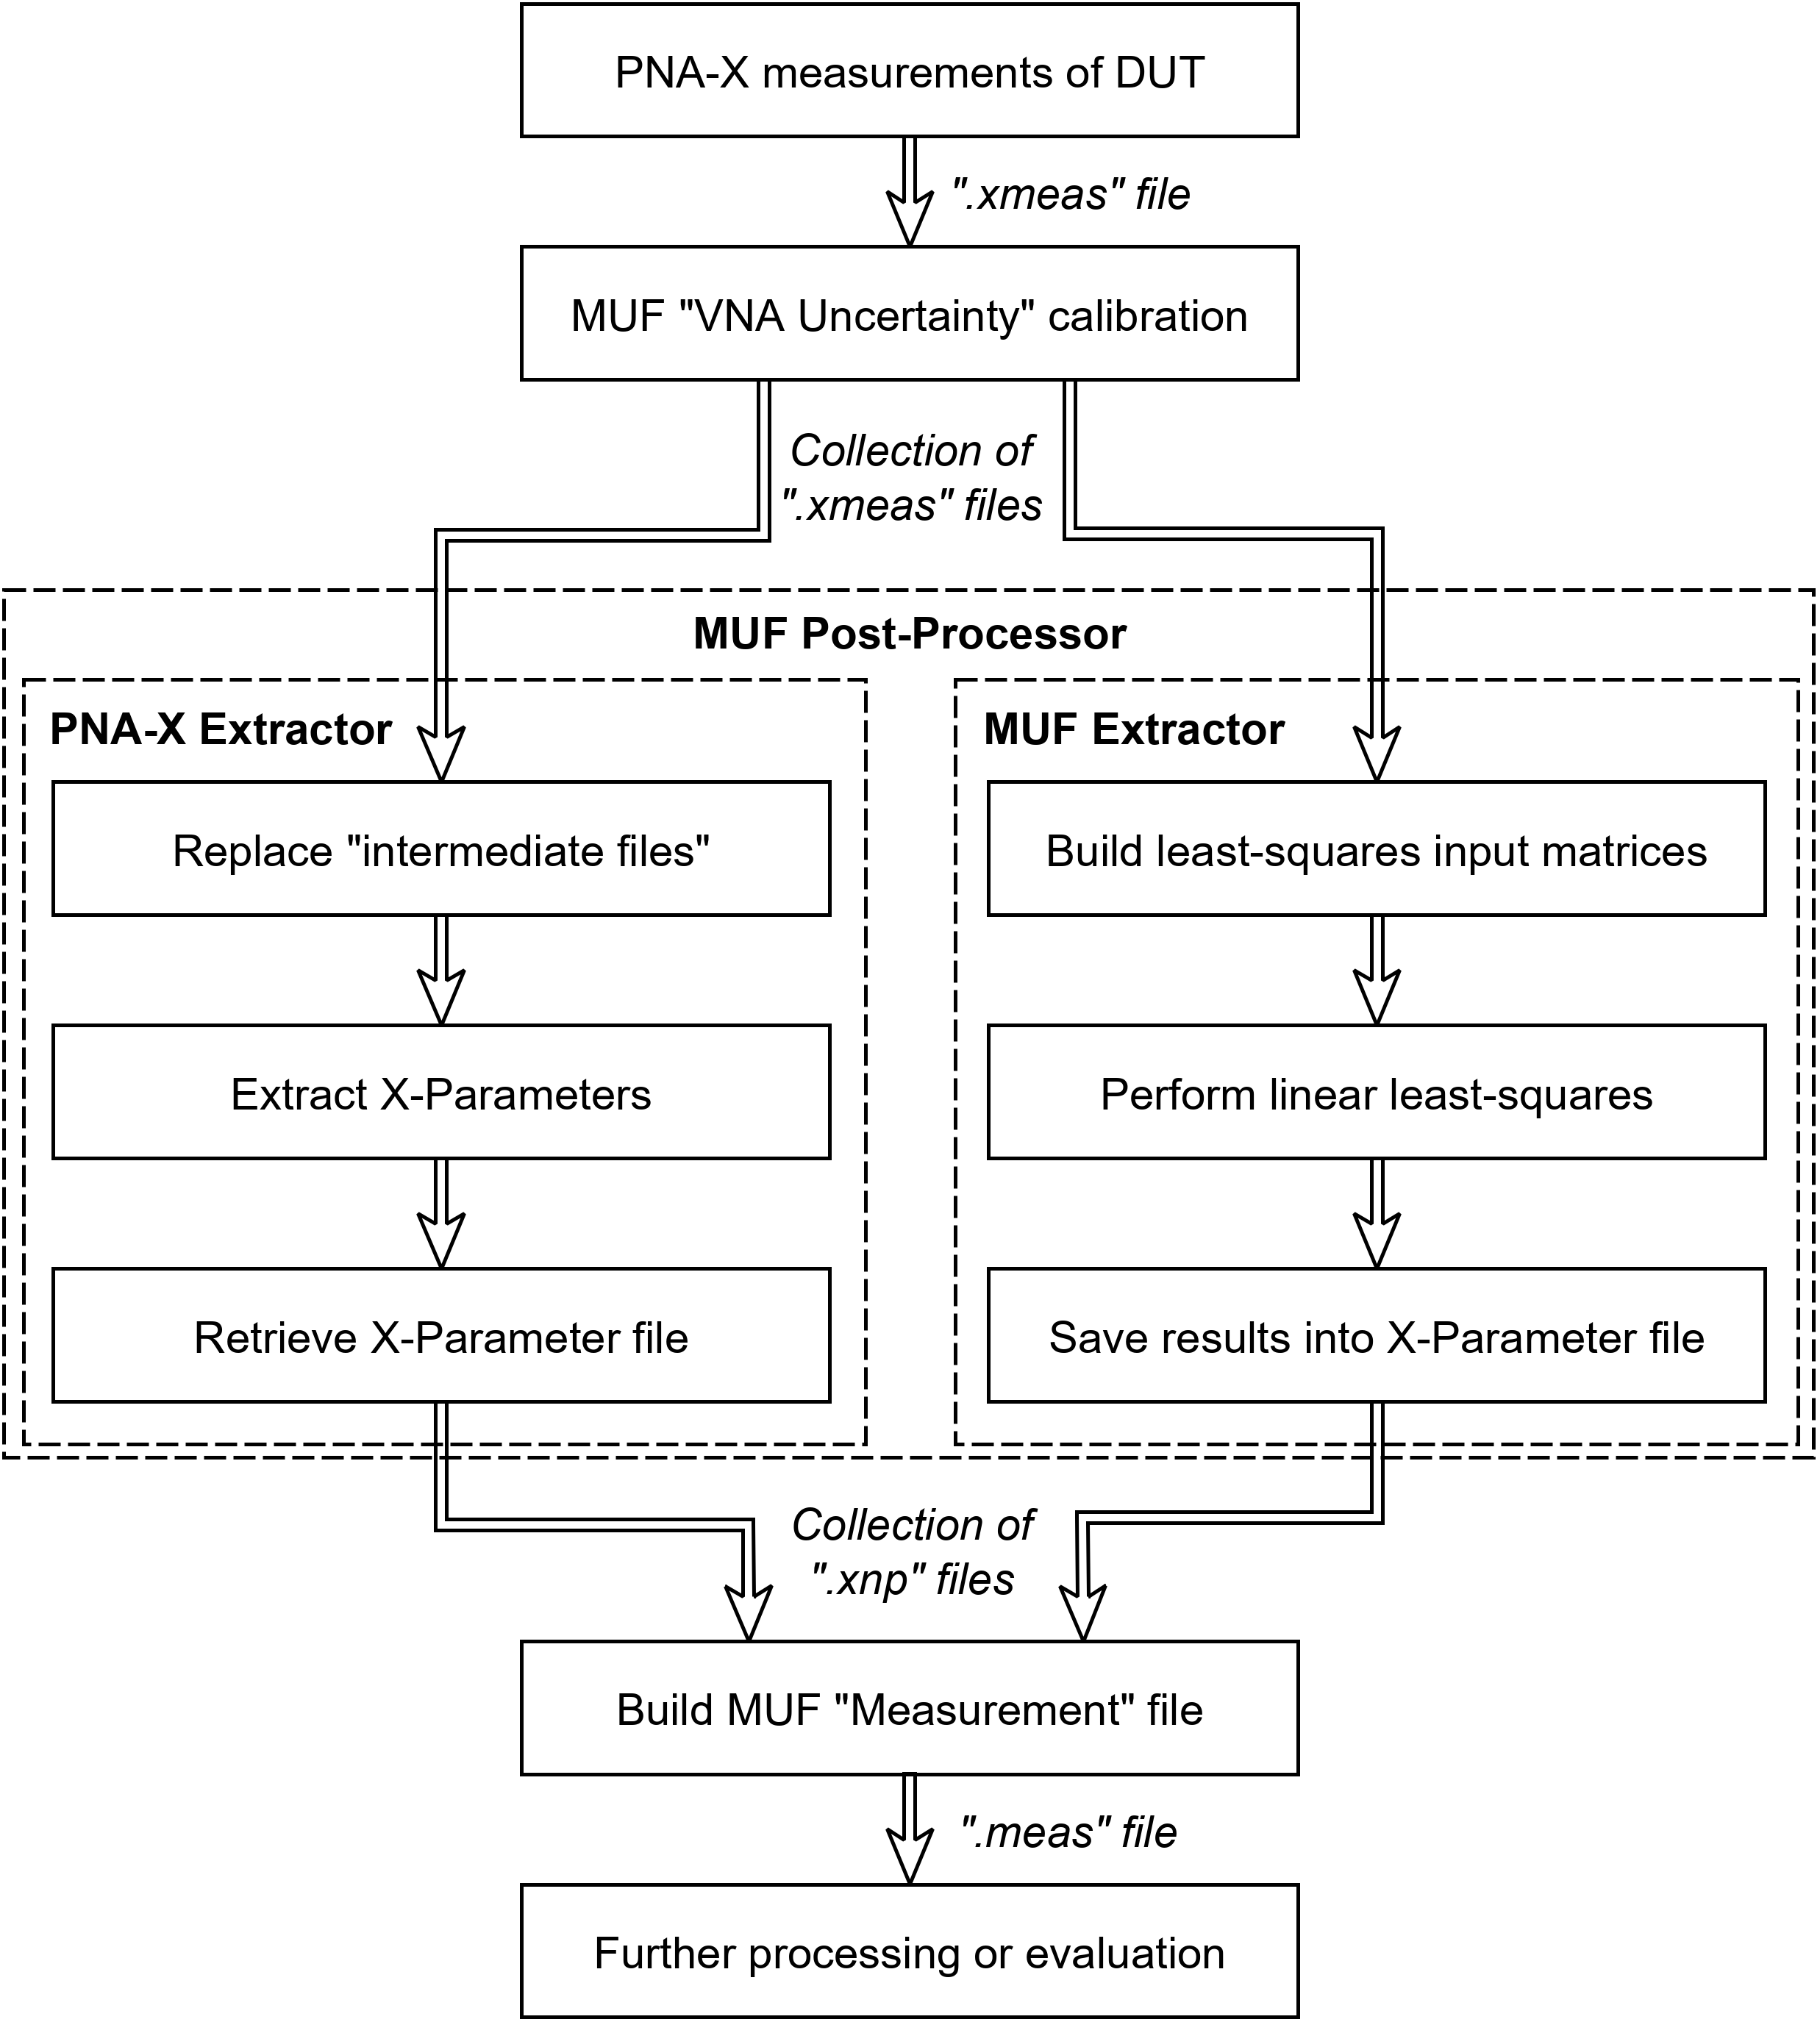
\includegraphics[width=0.9\textwidth]{uncproc}
	\caption[X-parameter uncertainty processing flow.]{Processing flow showing X-parameter extraction methods that are compatible with propagating uncertainty via numerical methods (i.e. Monte Carlo and sequential perturbation). Both the PNA-X and MUF extraction routines are called from a MUF post-processor which allows the user to select the desired approach. Both routines take X-parameter measurement files of the DUT as their input, and return X-parameter files.}
	\label{ch5_fig_uncproc}
\end{figure}

\subsubsection{PNA-X Extraction}

The PNA-X X-parameter measurement software is designed to guide the user through all steps of the process: calibration, device measurements and model extraction. Because the model extents (number of ports, harmonics, etc) are defined before measurement, the software will normally perform the X-parameter extraction immediately after the measurements have finished. This is desirable as it presents the user with visible plots of the parameters on the NVNA screen similar to traditional VNA measurements. There is no supported way to provide X-parameter measurements from a file and perform a stand-alone extraction. This is regrettable as it is the only way perturbed samples from the MUF uncertainty propagation can be processed into X-parameters and hence propagate the uncertainty further.

Fortunately, the software includes a somewhat esoteric feature which can be utilised to remove this limitation. Because the PNA-X hardware is limited on the amount of memory it can fit on a physically compact embedded computer, very large sweeps of measurements (as required for X-parameters extracted from load-pull experiments) can require more memory than is present. Therefore, because the X-parameters are extracted from the entire dataset, the software provides the ability to save ``intermediate files''  which are just subsets of the X-parameter measurements in ``.xmeas'' format.  The intention is that once the measurements are complete, the user immediately clicks on the option to ``Extract X-parameters from intermediate files'' and they are presented with the same end results as normal. Because the intermediate files are ASCII-encoded and not binary, it is possible to perform a dummy measurement (which initialises the file location), replace the intermediate file with a perturbed X-parameter measurement file processed by the MUF, and run the command to extract X-parameters. Through experimentation it has been found that the extraction routine only examines the supplied file, so the measurement setup used for the dummy measurement is not important and is chosen to minimise delay (i.e. sweeps containing a single point).

All of these steps can be performed remotely using the DCOM automation interface for the PNA-X \cite{DCOM}. The MUF Post-Processor software accepts a programming function as a measurement model and evaluates it against each numerical sample contained in input files produced by previous MUF processes. Therefore, the automated PNA-X extraction was implemented as a MUF post-processor which would transfer a sample to the PNA-X (via network and tested across the Atlantic!), request an extraction be performed, and retrieve the X-parameter results. The Post-Processor software then automatically builds a MUF Measurement file, which indexes all the propagated perturbed samples for future use or statistical evaluation.

\subsubsection{MUF Custom Post-Processor}

The alternative X-parameter extractor, which is ultimately incorporated into the same MUF post-processor as the PNA-X automation code as a different option, is based on the least-squares estimation presented earlier in this section. It should be said that the PNA-X algorithms may differ from that method, as they are intellectual property of Keysight and not openly available.

The implemented extractor was compared with the output from the PNA-X and mostly showed excellent agreement. There were some discrepancies with terms involving extraction tones applied at the fundamental frequency on port one, but these are expected as it is not known how the Keysight algorithm generates the LSOP value which is subtracted from these measurements. Keysight have also made it known that there is additional pre-processing of the measurements before X-parameter extraction in their algorithm. However, the few differences between extraction algorithms which occur are small enough (e.g. 1 dB at -50 dBm) that it is at least suitable for academic use in this project. With that being said, due to time constraints the MUF X-parameter extractor was only completed shortly before the end of this project, therefore all of the uncertainty propagation used in publications and this dissertation was performed with the PNA-X extractor.

\section{Evaluation of the Combined Standard Uncertainty of X-Parameters Extracted from Measurement Data}

The new uncertainty propagation described in the previous section was successfully applied to both a connectorised microwave amplifier (Mini-Circuits ZX60-14012L+ \cite{minicircuits}) and a surface-mount millimetre-wave amplifier mounted on an evaluation board with coaxial launches (Analog Devices HMC342LC4 \cite{hittite_amp}). Due to millimetre-wave amplifiers being a current research focus because of 5G infrastructure development, this amplifier was chosen as the example for a publication presenting the results of this project \cite{Stant_2018_TMTT}. Parts of this publication will be included in the remaining sections of this chapter. The experiment will now be described.

The MUF was used to perform the calibration of electromagnetic wave parameters measured using a Keysight  67 GHz N5247A PNA-X NVNA. The DUT \cite{hittite_amp} has a typical gain of 19 dB and a \mbox{1-dB} compression point at approximately 9 dBm output power at 25 GHz. To obtain results showing both the linear and nonlinear regimes of operation, the source power was swept between -22 dBm and -2 dBm in 0.25 dB steps. The fundamental frequency was set at 25 GHz, with a harmonic at 50 GHz also measured. The evaluation board used 2.92 mm precision connectors, connected via adapters to cables with 2.4 mm precision connectors. The calibration plane was located between the cables and the adapters (i.e. the adapters were included as part of the DUT), and the measurement setup had a nominal impedance of 50-$\Omega$. The intermediate frequency bandwidth (IFBW) was set to 10 Hz. The built-in X-parameter measurement routine was used and configured to extract cross-frequency terms between both harmonics using measurements at 4 extraction tone phases (this is the default setting). A photograph of the setup is shown in Figure \ref{ch5_fig_setup}.

\begin{figure}[t]
	\centering
	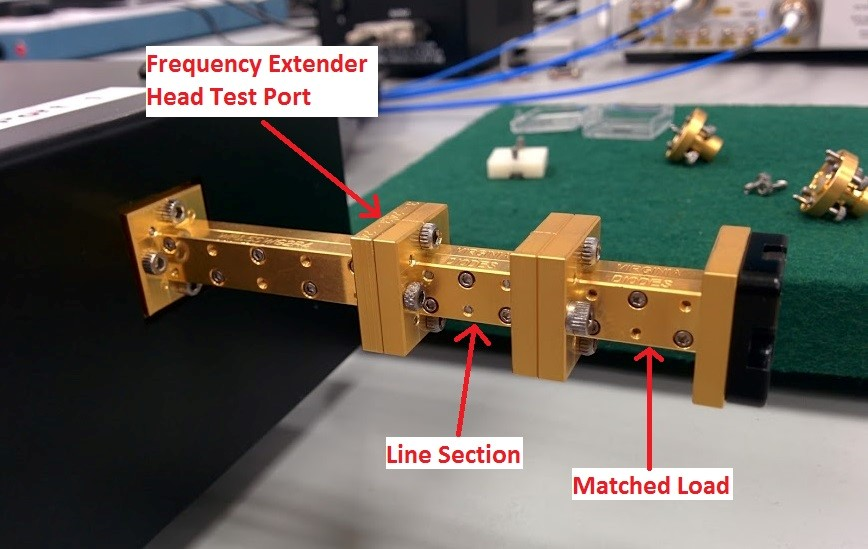
\includegraphics[width=\linewidth]{setup}
	\caption{The measurement setup used for extracting X-parameters from the DUT. Shown is the PNA-X LSNA (A), the phase reference comb generator (B), the phase calibration comb generator (C), the power meter (D), and the connected DUT (E).}
	\label{ch5_fig_setup}
\end{figure}

Uncertainties are propagated through all steps of the calibration by the MUF. Sources of uncertainty that were included covered the definitions and measurements of the passive calibration standards, the power meter calibration and measurement, the phase reference characterization and measurement, cable flexure, and connection repeatability of all calibration steps. Uncertainty due to random noise in the high-dynamic range receivers was omitted as it has been shown to be negligible with respect to that arising from other error sources in LSNA measurements \cite{Blockley_2007}.

The MUF supports several calibration algorithms, and for this measurement the multiline TRL calibration algorithm \cite{Engen_1979, Marks_1991} was chosen to allow direct dimensional traceability to national measurement standards. The calibration standards used were from a 1.85 mm precision coaxial calibration kit (Rosenberger RPC-1.85 LRL). Table \ref{ch5_table_passivestds} gives the dimensions of the line standards used for the calibration. To include the effect of connector repeatability on the passive calibration, each standard was measured several times with the connector oriented differently. These measurements were passed to the MUF program \textbf{Combine} which produces a mean value with an associated uncertainty.

\begin{table}[]
	\centering
	\caption{Nominal values and standard uncertainties for the TRL coaxial line standards.}
	\label{ch5_table_passivestds}
	\begin{tabular}{ccc}
		\hline
		Dimension         & Line 1 value (mm) & Line 2 value (mm) \\ \hline
		Line length       & 13.004 $\pm$ 0.003 & 14.913 $\pm$ 0.003 \\
		Line inside dia.  & 0.803 $\pm$ 0.001 & 0.803 $\pm$ 0.008 \\
		Line outside dia. & 1.850 $\pm$ 0.005 & 1.850 $\pm$ 0.005 \\ \hline            
	\end{tabular}
\end{table}

The calibration model for the power meter itself is defined in \cite{Keysight_2017} and includes the reference oscillator mismatch, the reference oscillator power uncertainty, the zero-set error, the zero carry-over error, the instrumentation error, and error in the power sensor calibration factor. The estimates and uncertainties used for these parameters in the calibration are shown in Table \ref{ch5_table_powerunc} and are derived from specifications supplied by the manufacturer. The mismatch of the power sensor was also measured using a calibrated VNA and included in the absolute calibration. Connector repeatability was assessed for this measurement in the same way as for the passive standards.

\begin{table}[]
	\centering
	\caption{Standard uncertainties for power meter uncertainty contributions derived in \cite{Keysight_2017}}
	\label{ch5_table_powerunc}
	\begin{tabular}{cc}
		\hline
		Contribution                           & Standard uncertainty \\ \hline
		Reference oscillator mismatch          & 0.2\%                \\
		Reference oscillator power uncertainty & 0.6\%                \\
		Zero-set error                         & 0.5\% meter full scale \\
		Zero carry-over error                  & 0.2\% meter full scale \\
		Instrumentation error                  & 0.5\% meter full scale \\
		Calibration factor error               & 0.024               \\ \hline
	\end{tabular}
\end{table}

The two phase references used for both calibration and synchronisation of the mixer-based NVNA were Keysight 67 GHz comb generators\cite{Keysight_2014}. The phase uncertainties for the calibration phase reference are given in Table \ref{ch5_table_phaseunc} and were obtained through characterization with a sampling oscilloscope at NIST, which is traceable to national measurement standards via electro-optic calibration \cite{Reader_2008, Hale_2009} as described in Chapter 4.

\begin{table}[]
	\centering
	\caption{Nominal phase and standard uncertainty for harmonic phase reference at calibration frequencies}
	\label{ch5_table_phaseunc}
	\begin{tabular}{ccc}
		\hline
		Frequency (GHz) & Characterized phase (deg.) & Measured phase (deg.)\\ \hline
		25 & 181.5 $\pm$ 0.4 & -16.8 $\pm$ 1.5 \\ 
		50 & 170.8 $\pm$ 1.0 & 61.0 $\pm$ 2.5 \\ 
		\hline
	\end{tabular}
\end{table}

\subsection{X-Parameter Uncertainties}

In this example we used Monte Carlo with 1000 samples to propagate uncertainty to the X-parameters of the DUT. This required 8 hours of processing for the calibration and a further 8 hours of processing for the X-parameter extraction. A histogram is provided in Figure \ref{ch5_fig_hist} showing good agreement between the Monte Carlo and sensitivity analysis. This level of agreement is typical for all of the extracted X-parameters.

The estimated values and standard uncertainties from the Monte Carlo analysis for the magnitude and phase of a sample of X-parameter terms are shown in Figure \ref{ch5_fig_summaryplots}. It can be seen in all plots that there is a clear change in uncertainty for several X-parameters as the DUT transitions between the linear and nonlinear regimes.

The phase noise seen at lower powers in the estimate of $X^\textrm{T}_{2,1;2,2}$ is not accompanied by an increase in measurement uncertainty. This suggests that it arises from the extraction routine, which contributes another source of uncertainty not studied in this project. By design, the $X^\textrm{T}$ parameters are negligible in the linear regime, and so this effect will have little contribution when the model is used.

\begin{figure}
	\centering
	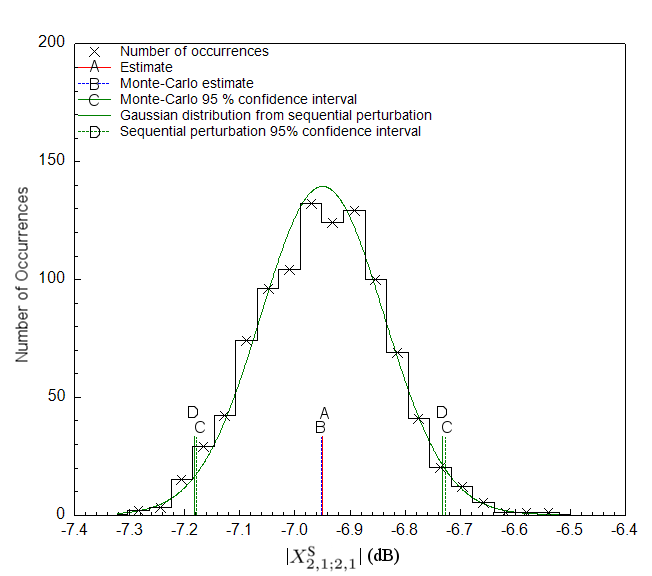
\includegraphics[width=0.8\textwidth]{hist}
	\caption{Histogram comparing the Monte Carlo and sequential perturbation uncertainty results for $X^\textrm{S}_{2,1;2,1}$ (25 GHz) of the DUT at -2.4 dBm source power. The vertical line in the center of the plot (A) shows the nominal value (estimate), (B) shows the Monte Carlo average, and (C, D) show the Monte Carlo and sequential perturbation 95\% confidence intervals, respectively.}
	\label{ch5_fig_hist}
\end{figure}

\begin{figure}
	\centering
	\begin{subfigure}{0.45\textwidth}
		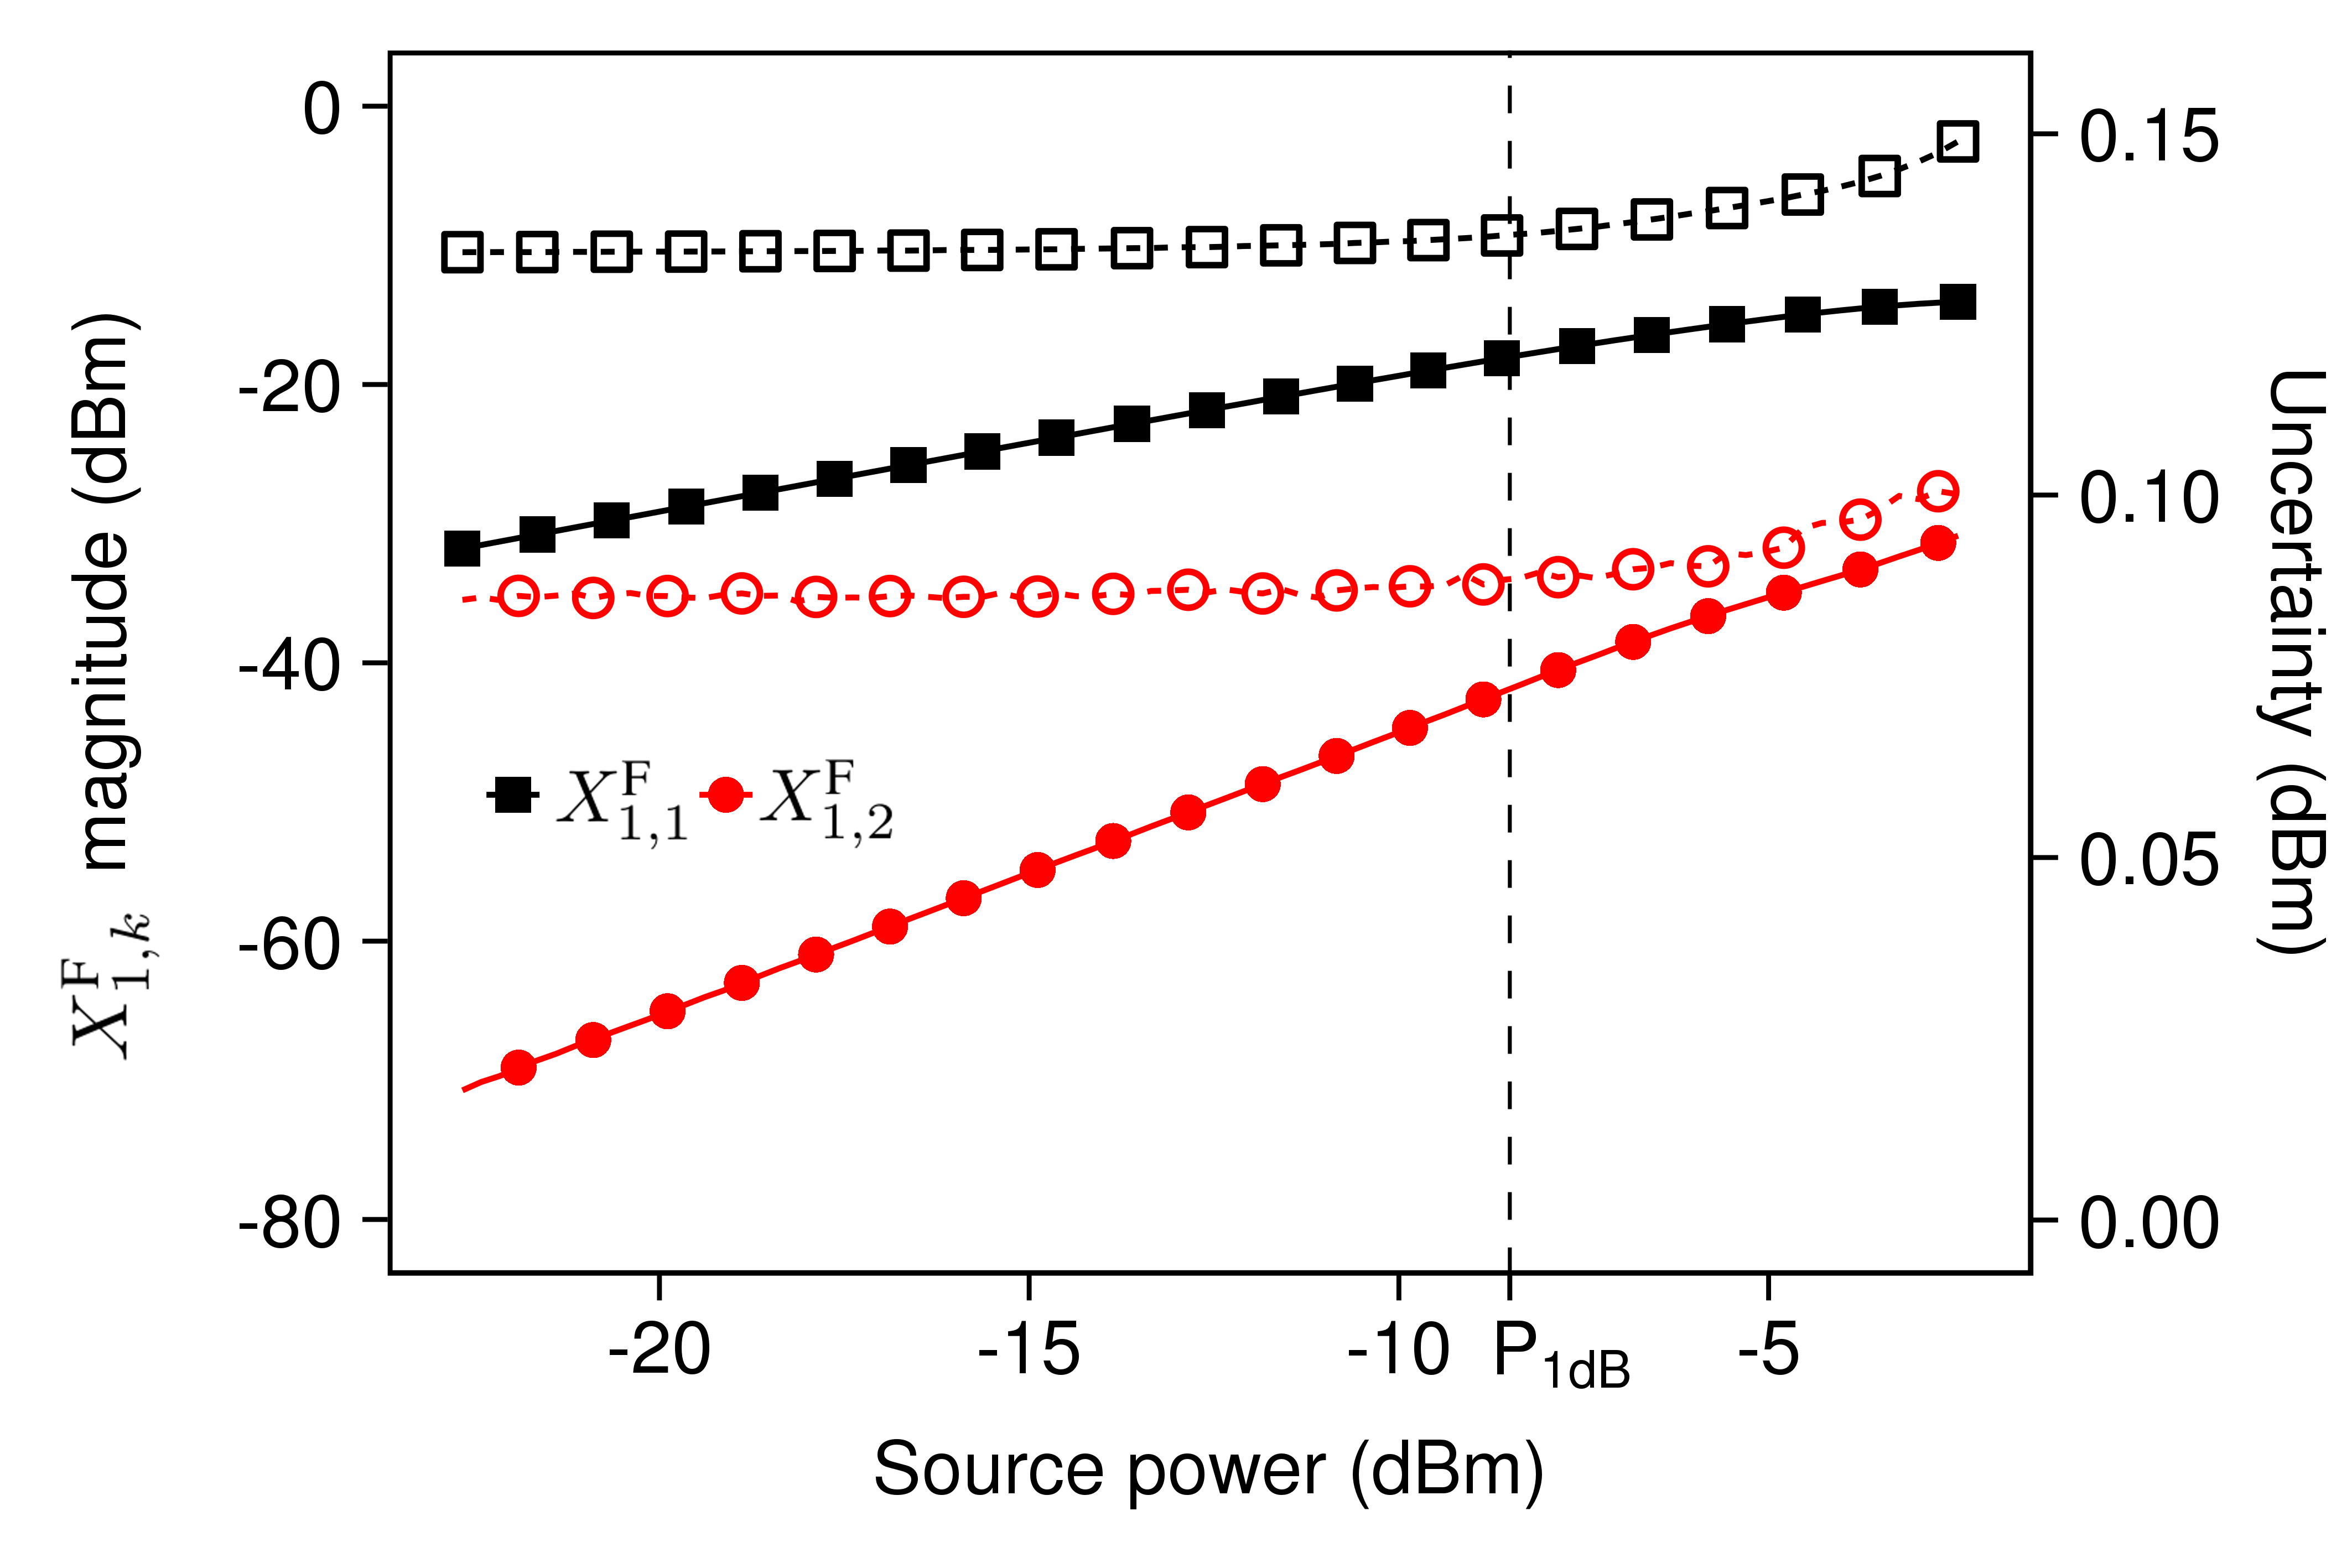
\includegraphics[width=\linewidth,height=5cm]{fig4a}			
		\label{ch5_fig_FB1kdB}
	\end{subfigure}\hfil%
	\begin{subfigure}{0.45\textwidth}
		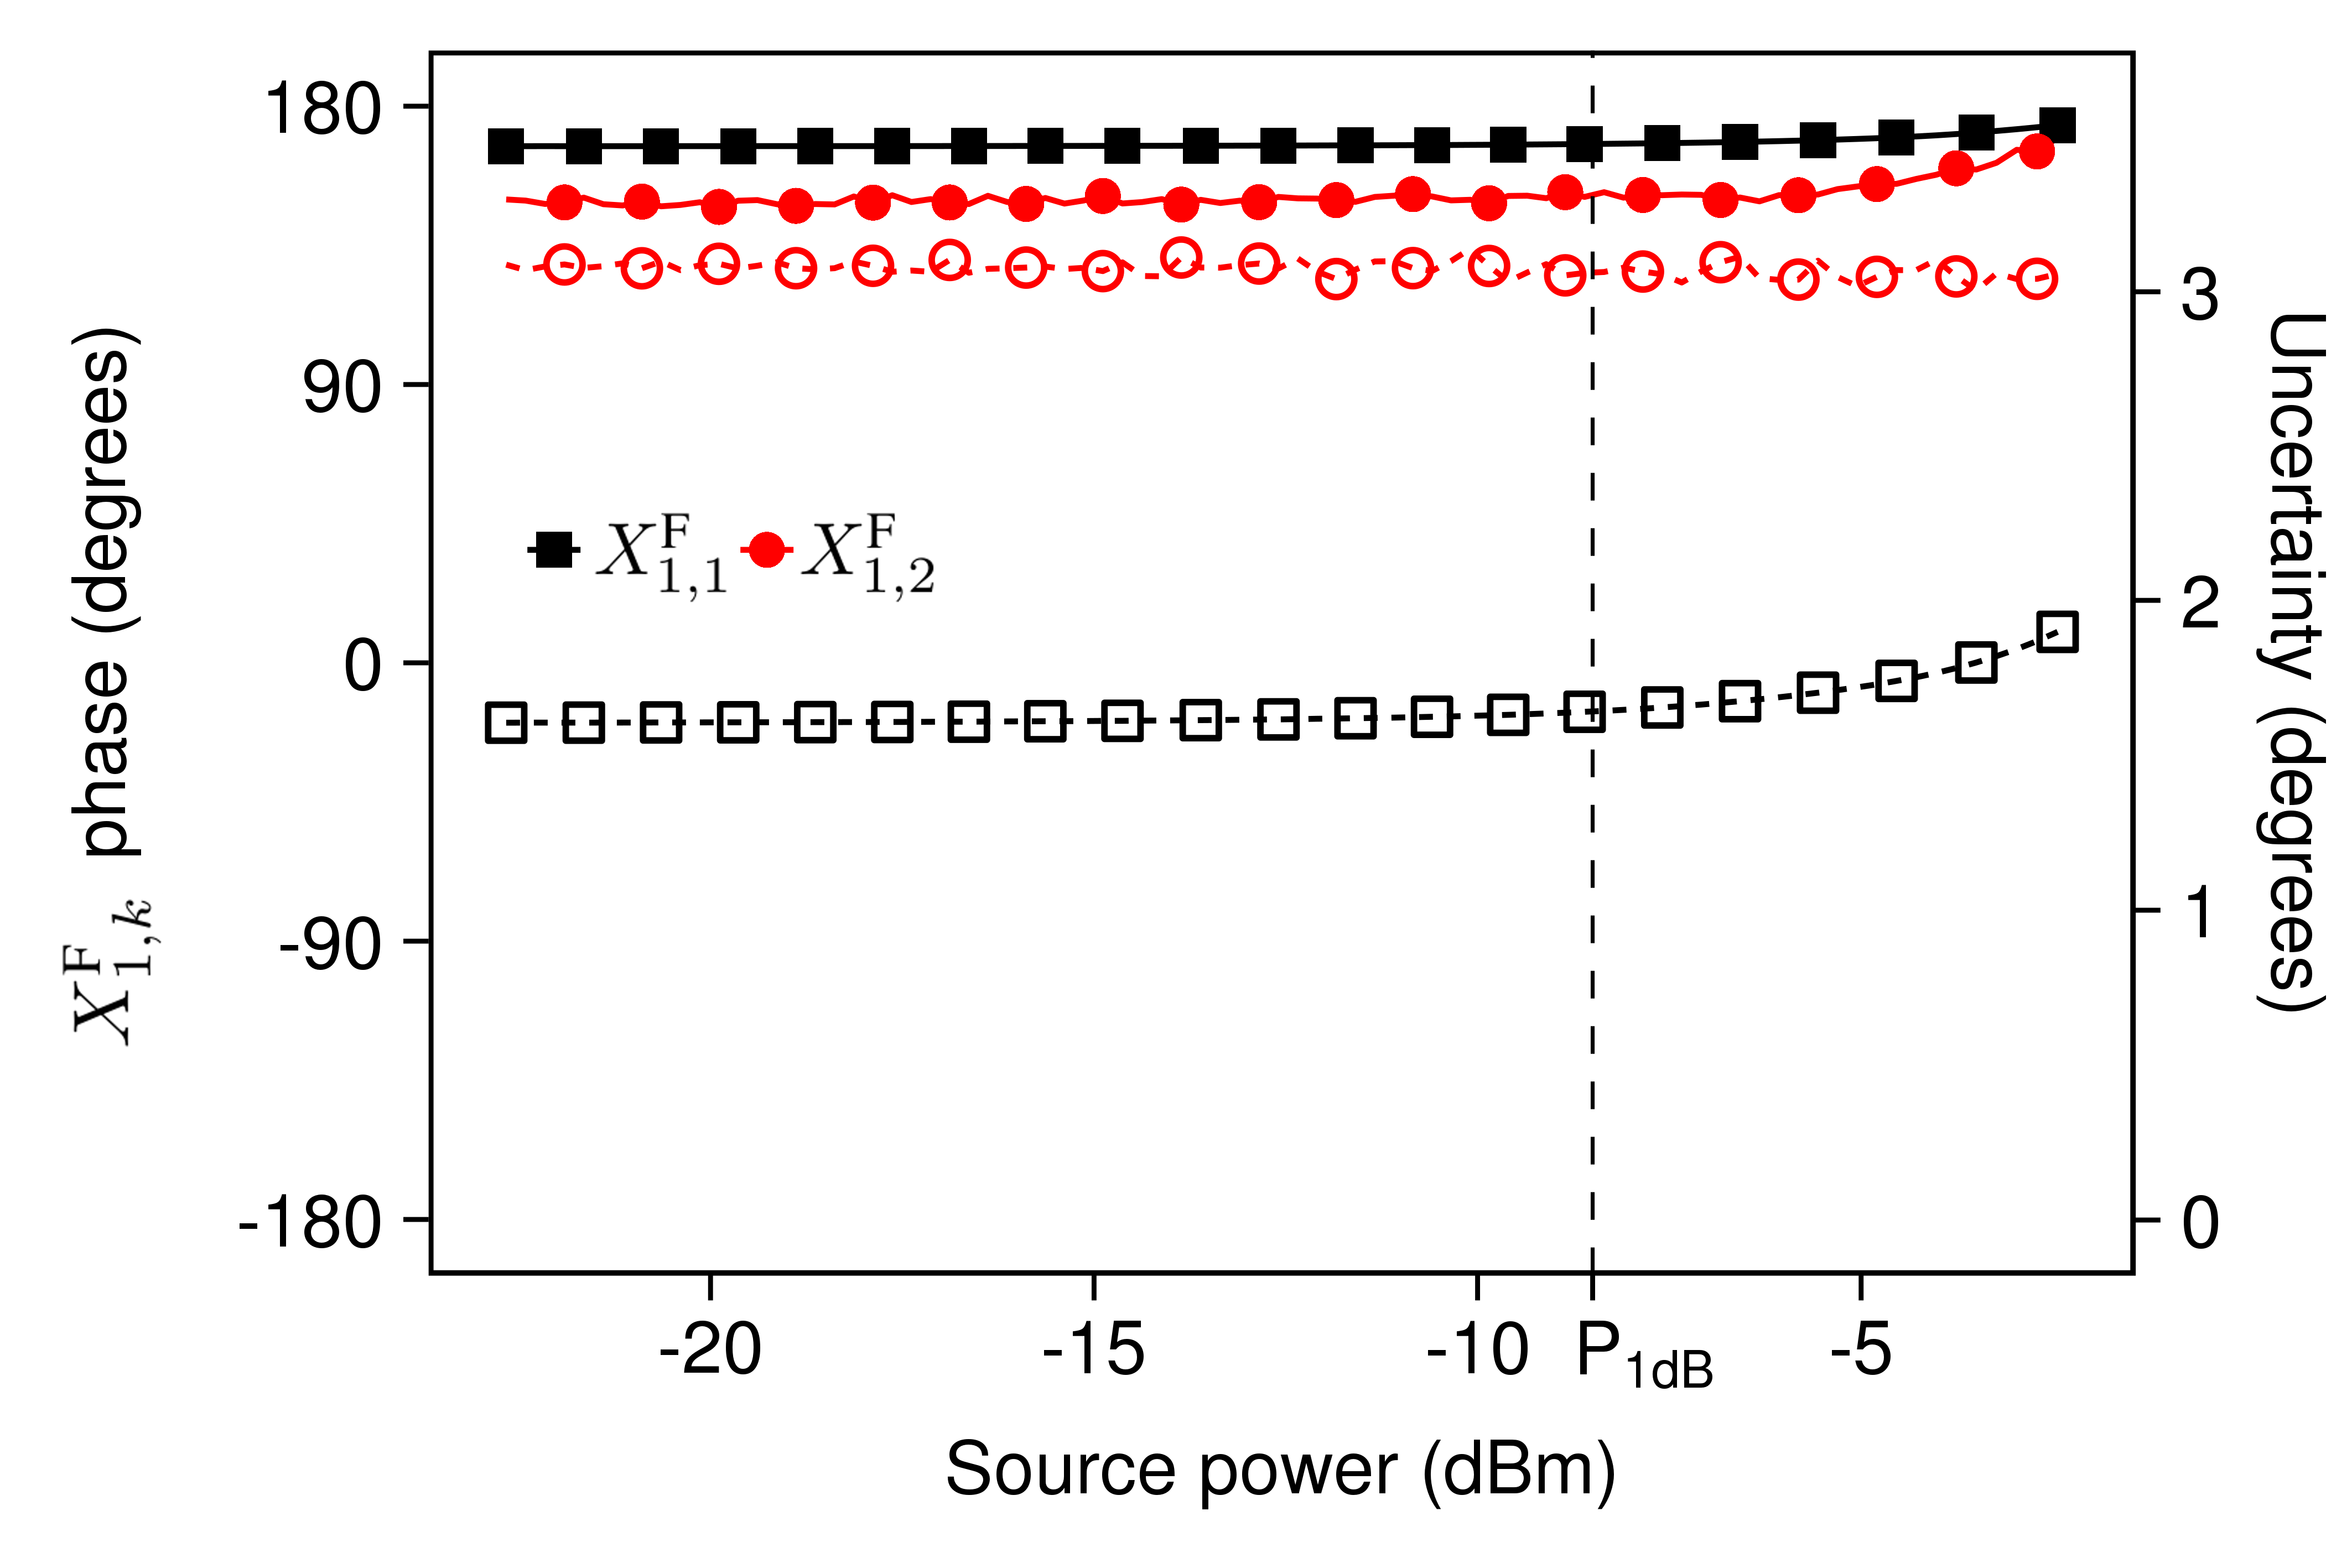
\includegraphics[width=\linewidth,height=5cm]{fig4b}
		\label{ch5_fig_FB1kp}
	\end{subfigure}
	\begin{subfigure}{0.45\textwidth}
		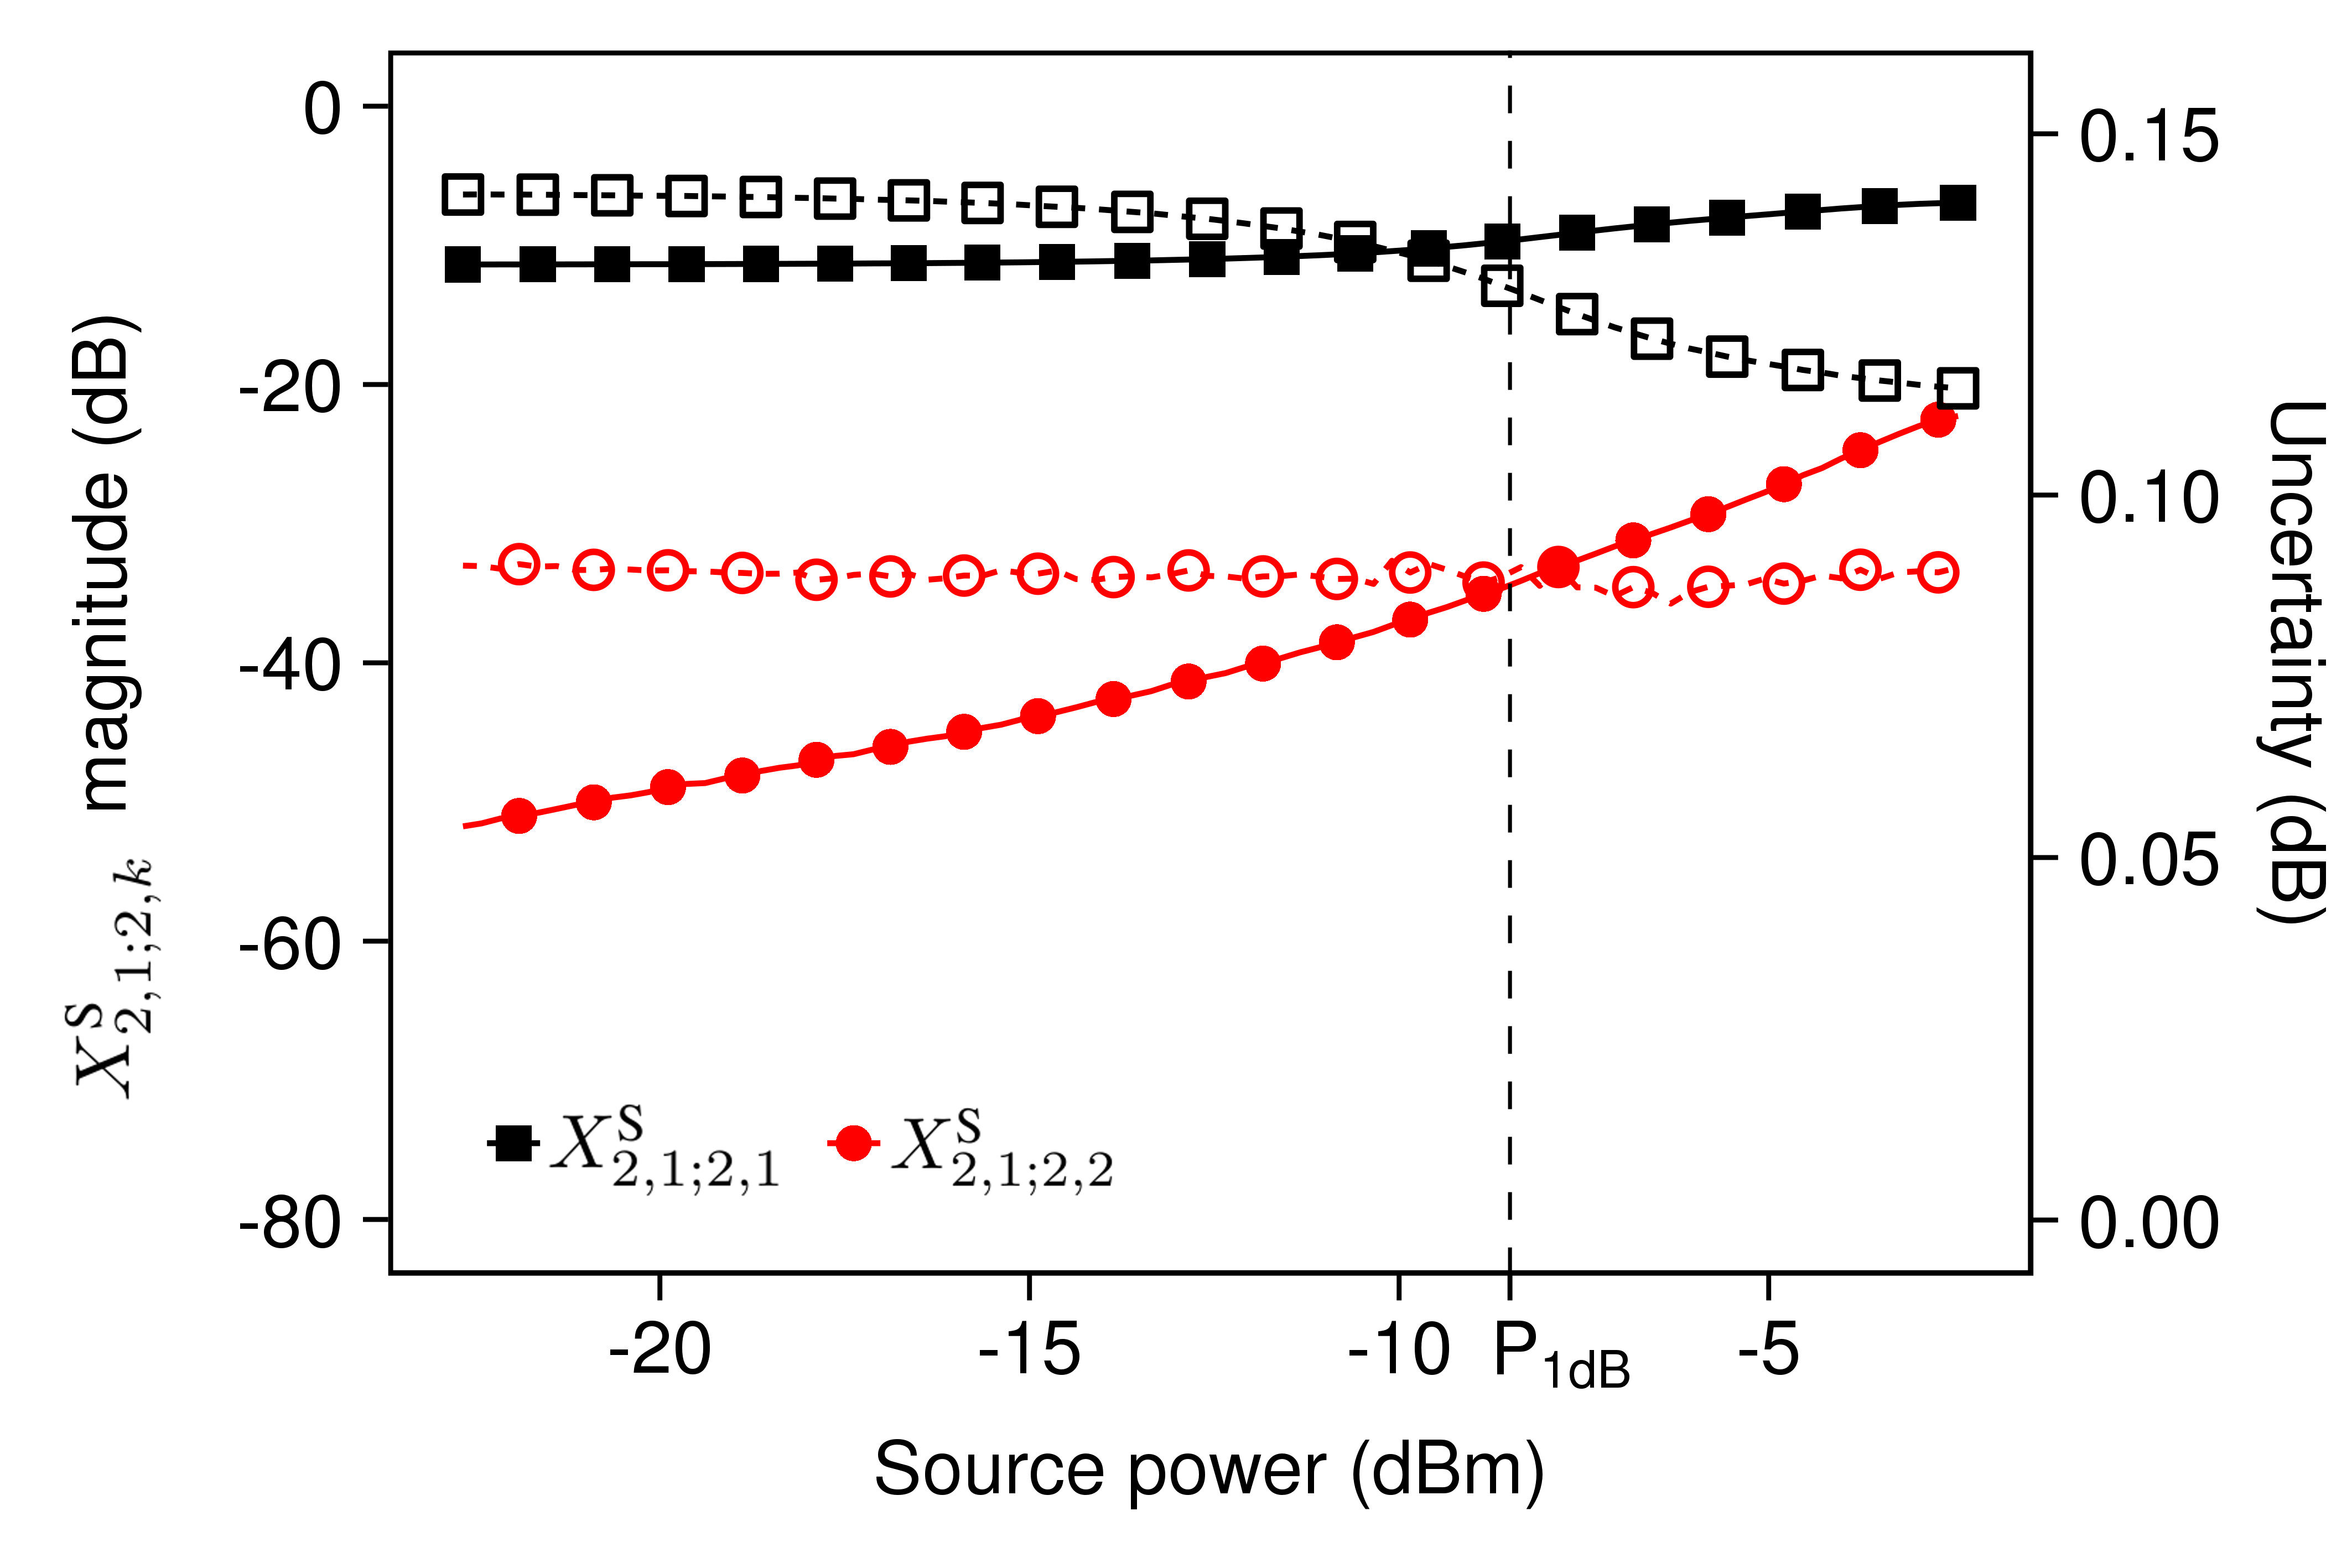
\includegraphics[width=\linewidth,height=5cm]{fig4c}
		\label{ch5_fig_s212kdB}
	\end{subfigure}\hfil%
	\begin{subfigure}{0.45\textwidth}
		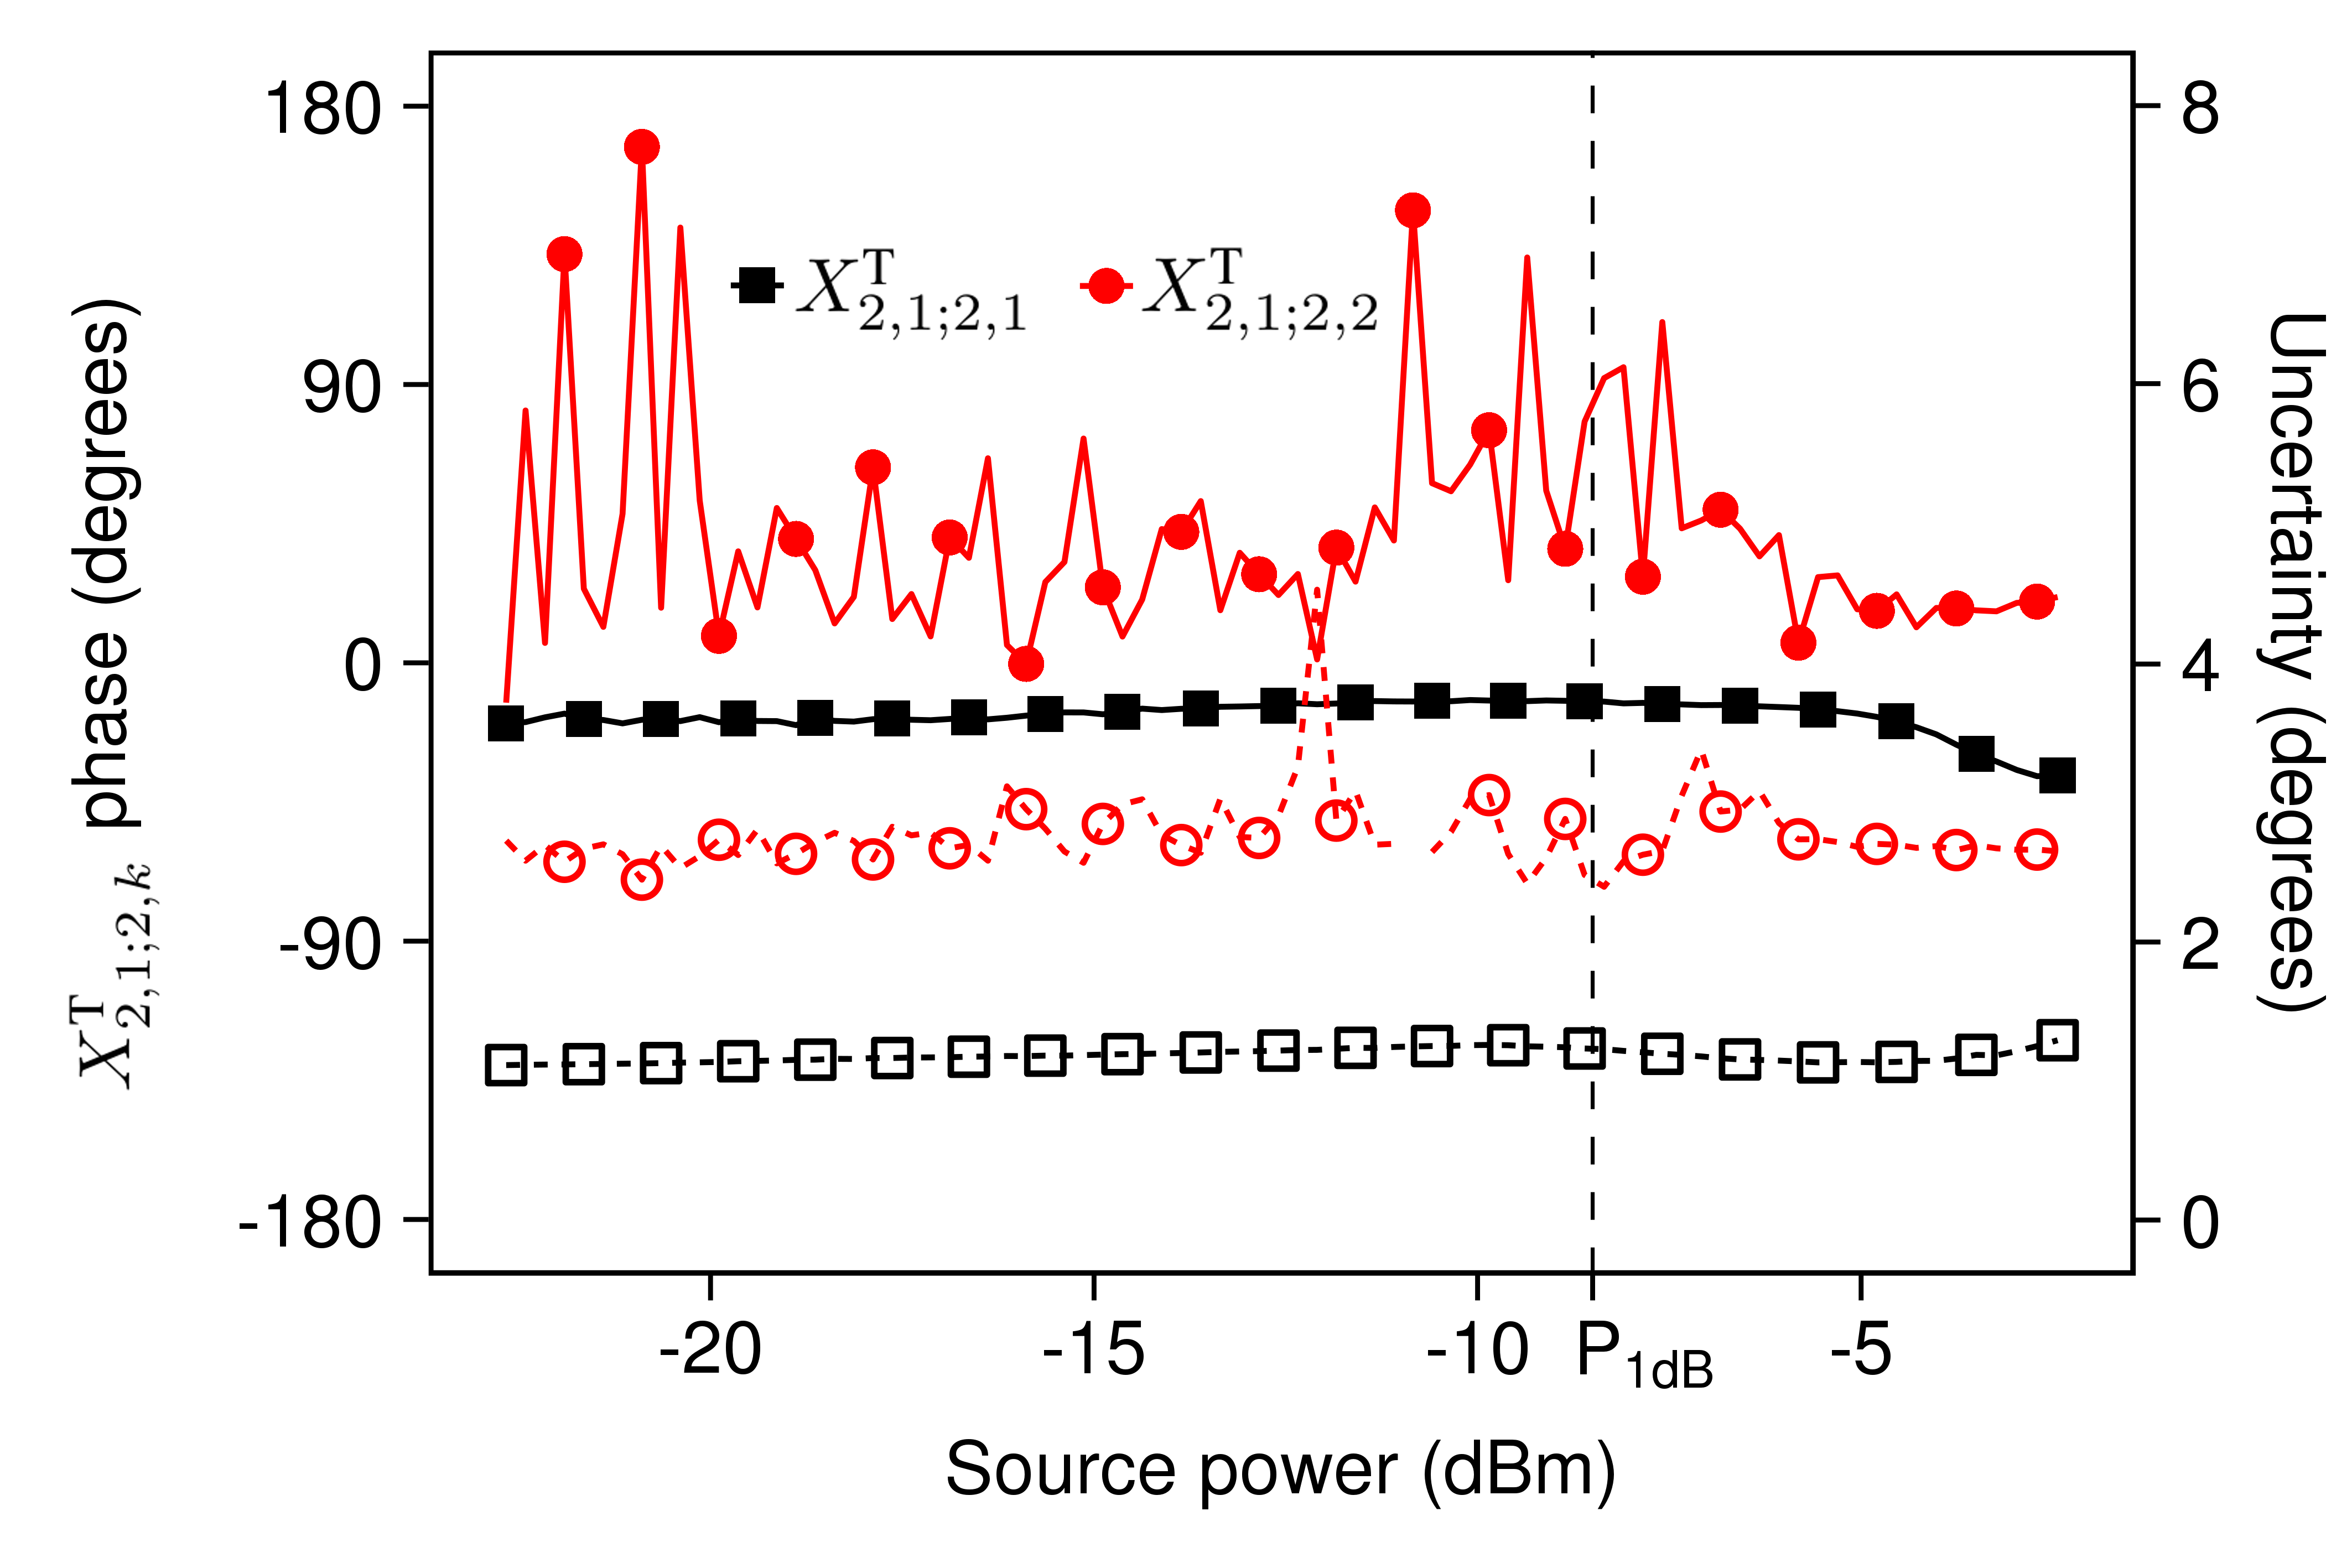
\includegraphics[width=\linewidth,height=5cm]{fig4d}	
		\label{ch5_fig_t212kp}
	\end{subfigure}
	\caption{Estimates (solid line and shapes, left scale) and standard uncertainties (dashed line and hollow shapes, right scale) for the magnitude and phase of a sample of the extracted X-parameters. Harmonic indices 1 and 2 relate to measurement frequencies of 25 and 50 GHz, respectively. Uncertainties are a linear variation of the scale value.}
	\label{ch5_fig_summaryplots}
\end{figure}

\subsection{Sensitivity Analysis for X-parameter Uncertainties}

\figurename{ \ref{fig:sensplots}} shows a sample of the sensitivity analysis results for the X-parameter uncertainty obtained using sequential perturbation. Because over 300 sources of uncertainty were included in the analysis they have been grouped for clarity.

It can be seen that the power calibration has a dominant contribution to the uncertainty in the magnitude of $X^F_{12}$. This is to be expected because the $X^F$ terms represent the absolute electromagnetic waves output from the DUT, and the uncertainties from the power meter in the LSNA calibration (i.e. in the corrected wave measurements) are significantly larger than those from the TRL standards.

The TRL calibration uncertainty is also a dominant contribution to the uncertainty in the magnitude of most of the small-signal $X^\textrm{S}$ and $X^\textrm{T}$ terms. Because these terms are similar to S-parameters, in that they represent a ratio between electromagnetic waves, any correlated error components are cancelled. Both the power and phase calibration errors are correlated for terms concerning a single frequency, but only power calibration errors appear to be correlated for cross-frequency terms. This can be seen from the lack of uncertainty contribution from the phase calibration to the $X^\textrm{T}_{2,1;2,1}$ term.

For these example measurements, it can also be seen that the uncertainty contribution from cable flexure (and reconnection) was significant in all results. This is a well-known issue for electromagnetic measurements at millimeter-wave frequencies and above. This uncertainty contribution could be reduced by further limiting cable movement using mechanical fixturing.

\begin{figure}
	\centering
	\begin{subfigure}{0.45\textwidth}
		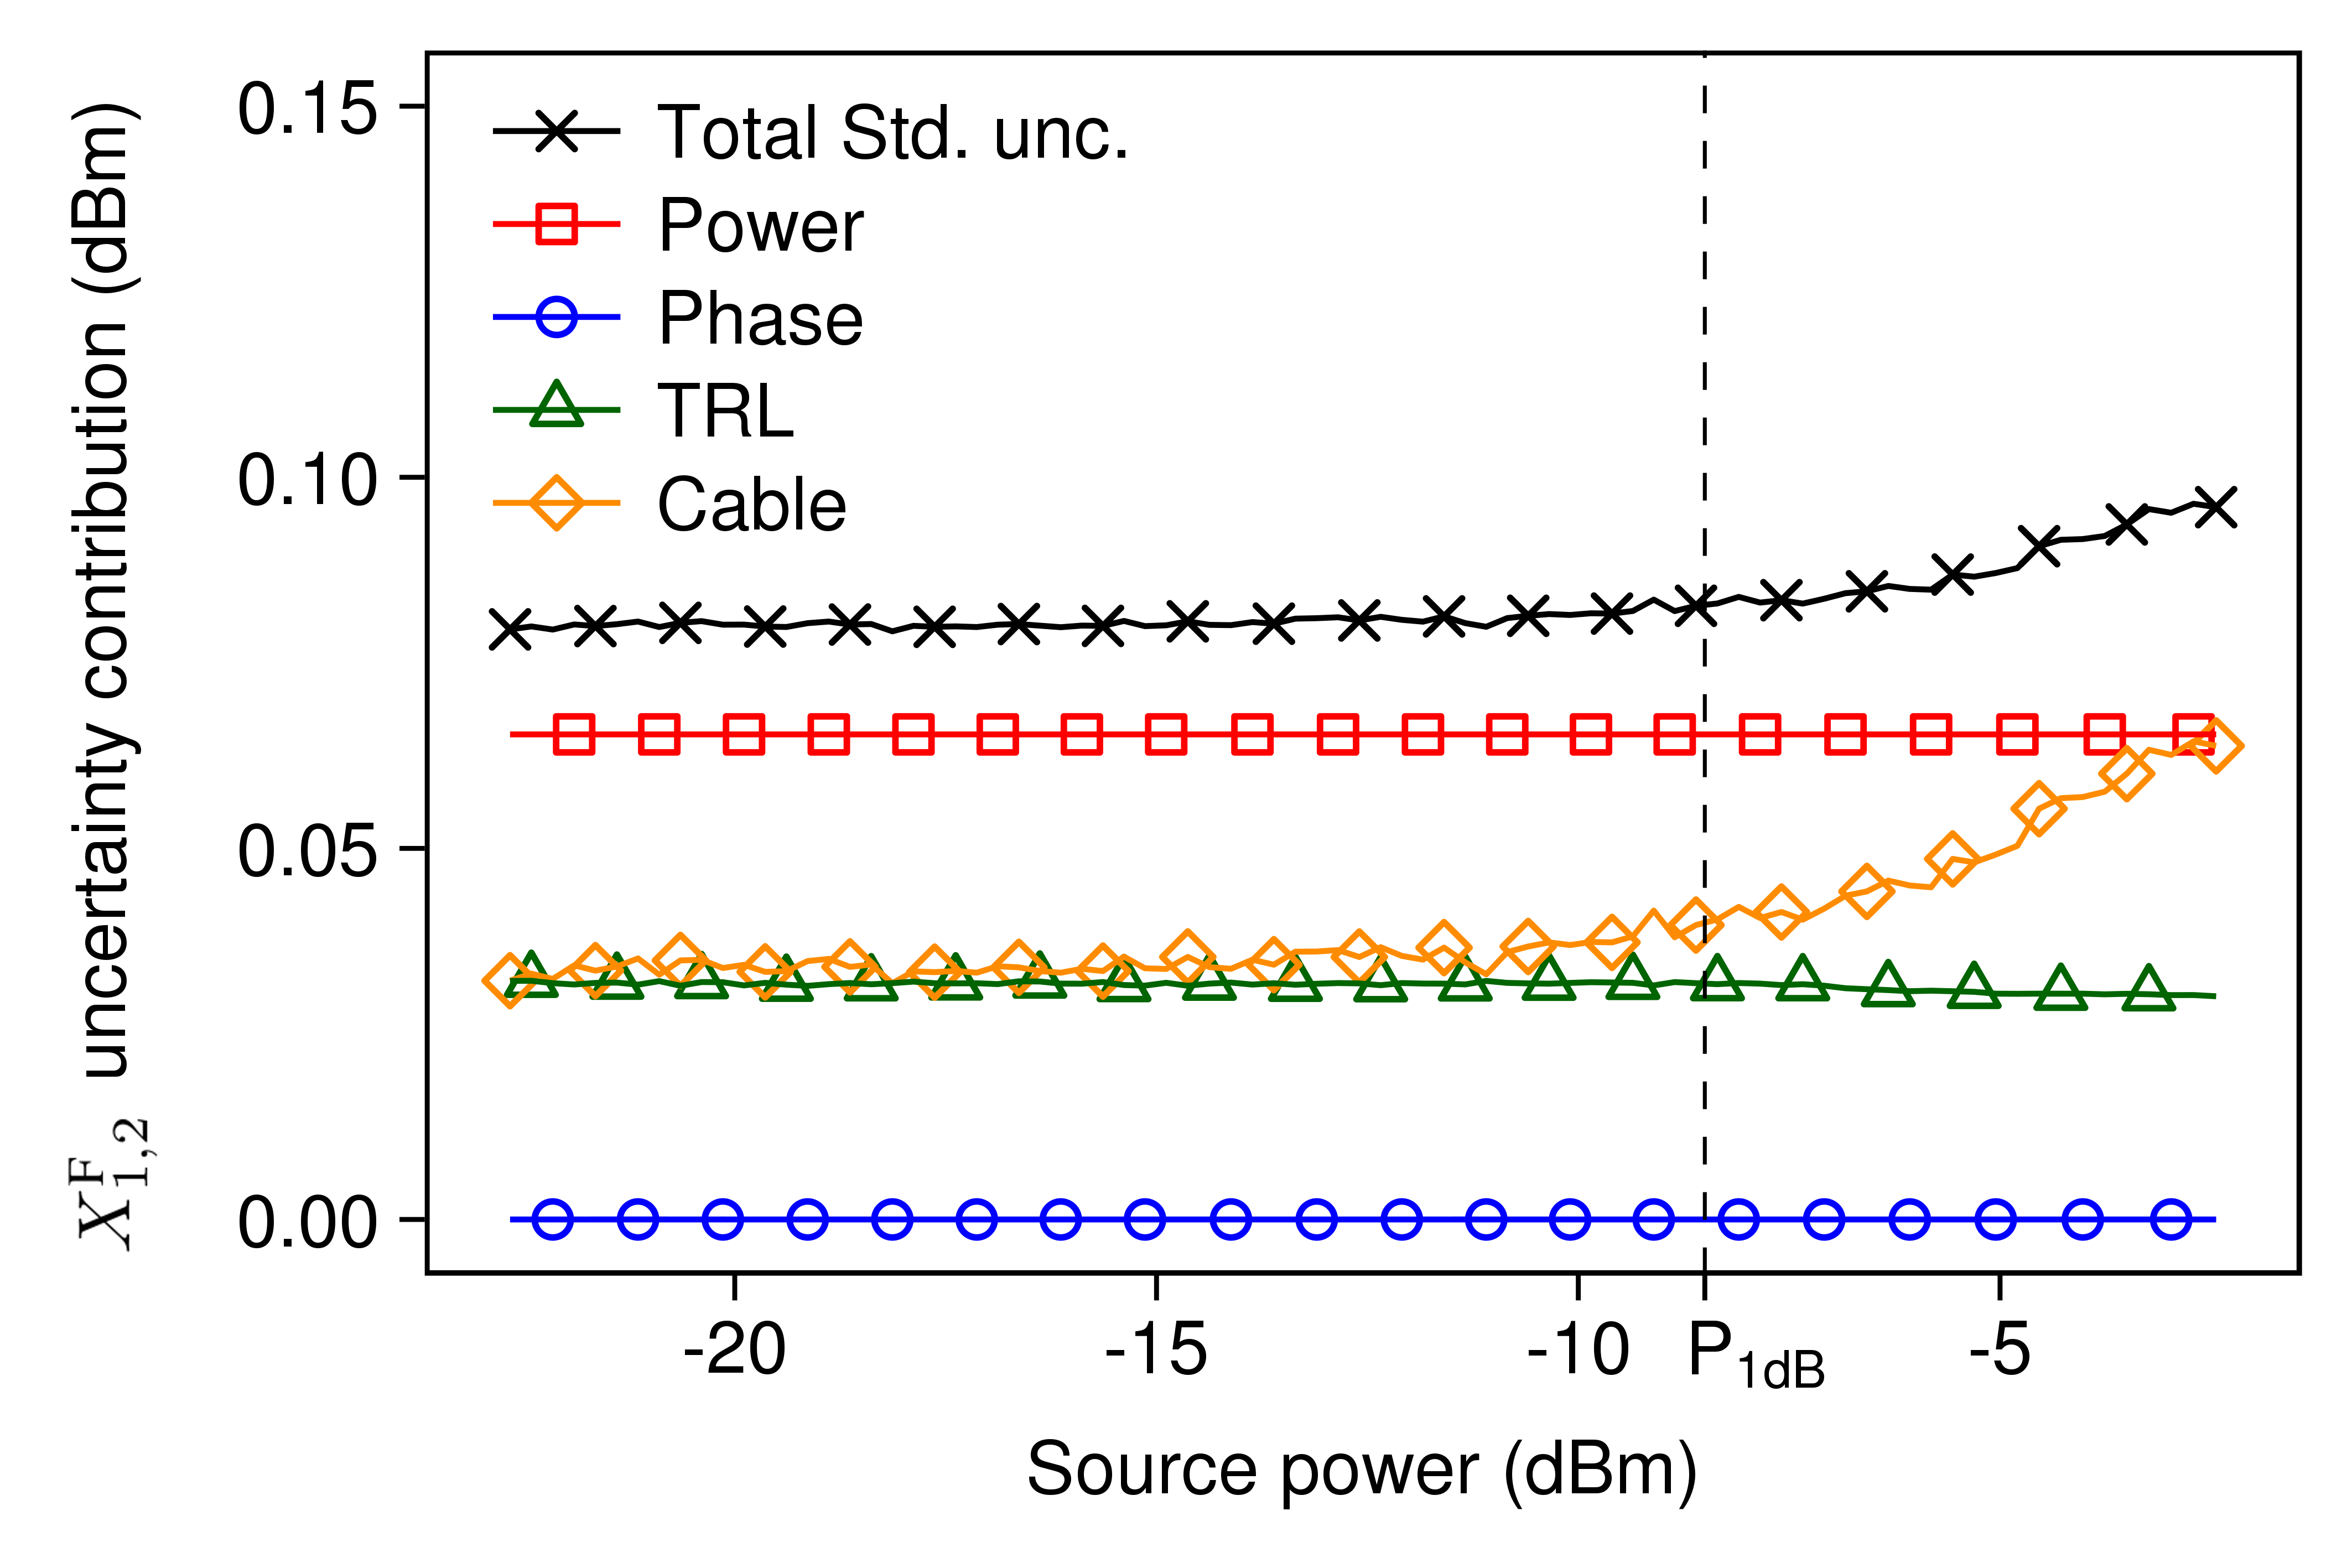
\includegraphics[width=\linewidth,height=5cm]{fig5a}			
		\label{ch5_fig_fb12magsens}
	\end{subfigure}\hfil%
	\begin{subfigure}{0.45\textwidth}
		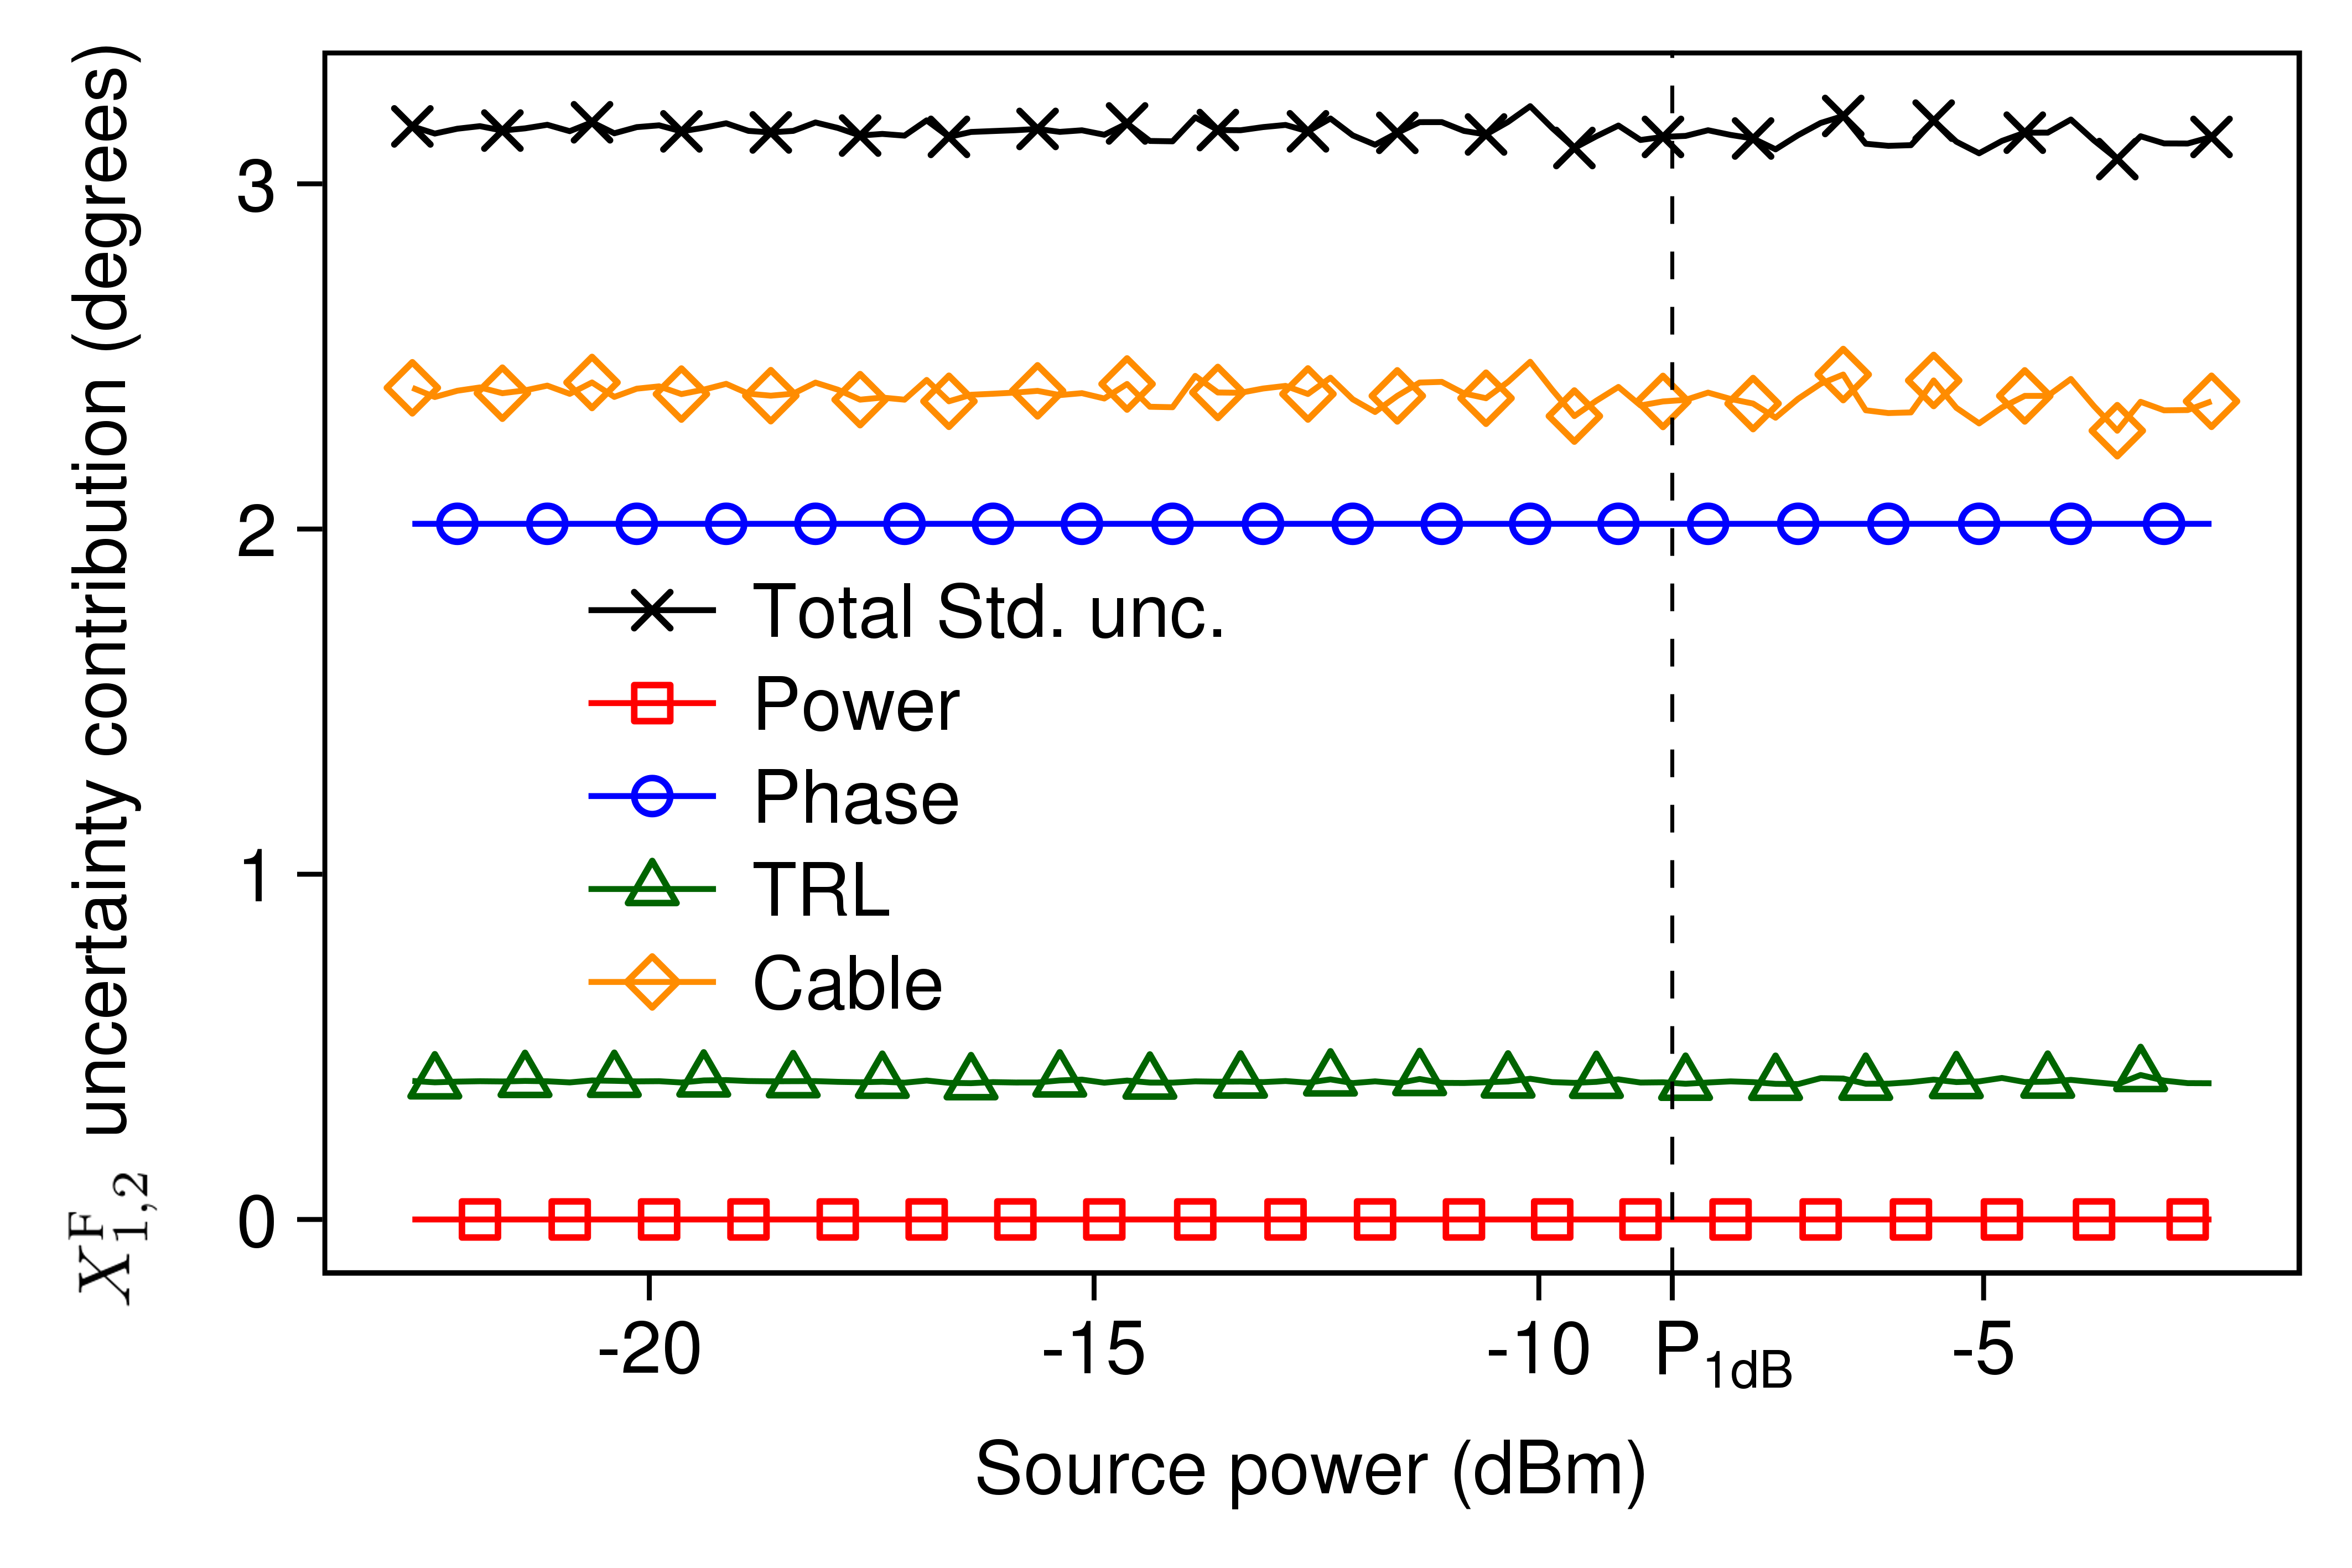
\includegraphics[width=\linewidth,height=5cm]{fig5b}
		\label{ch5_fig_fb12phasesens}
	\end{subfigure}
	\begin{subfigure}{0.45\textwidth}
		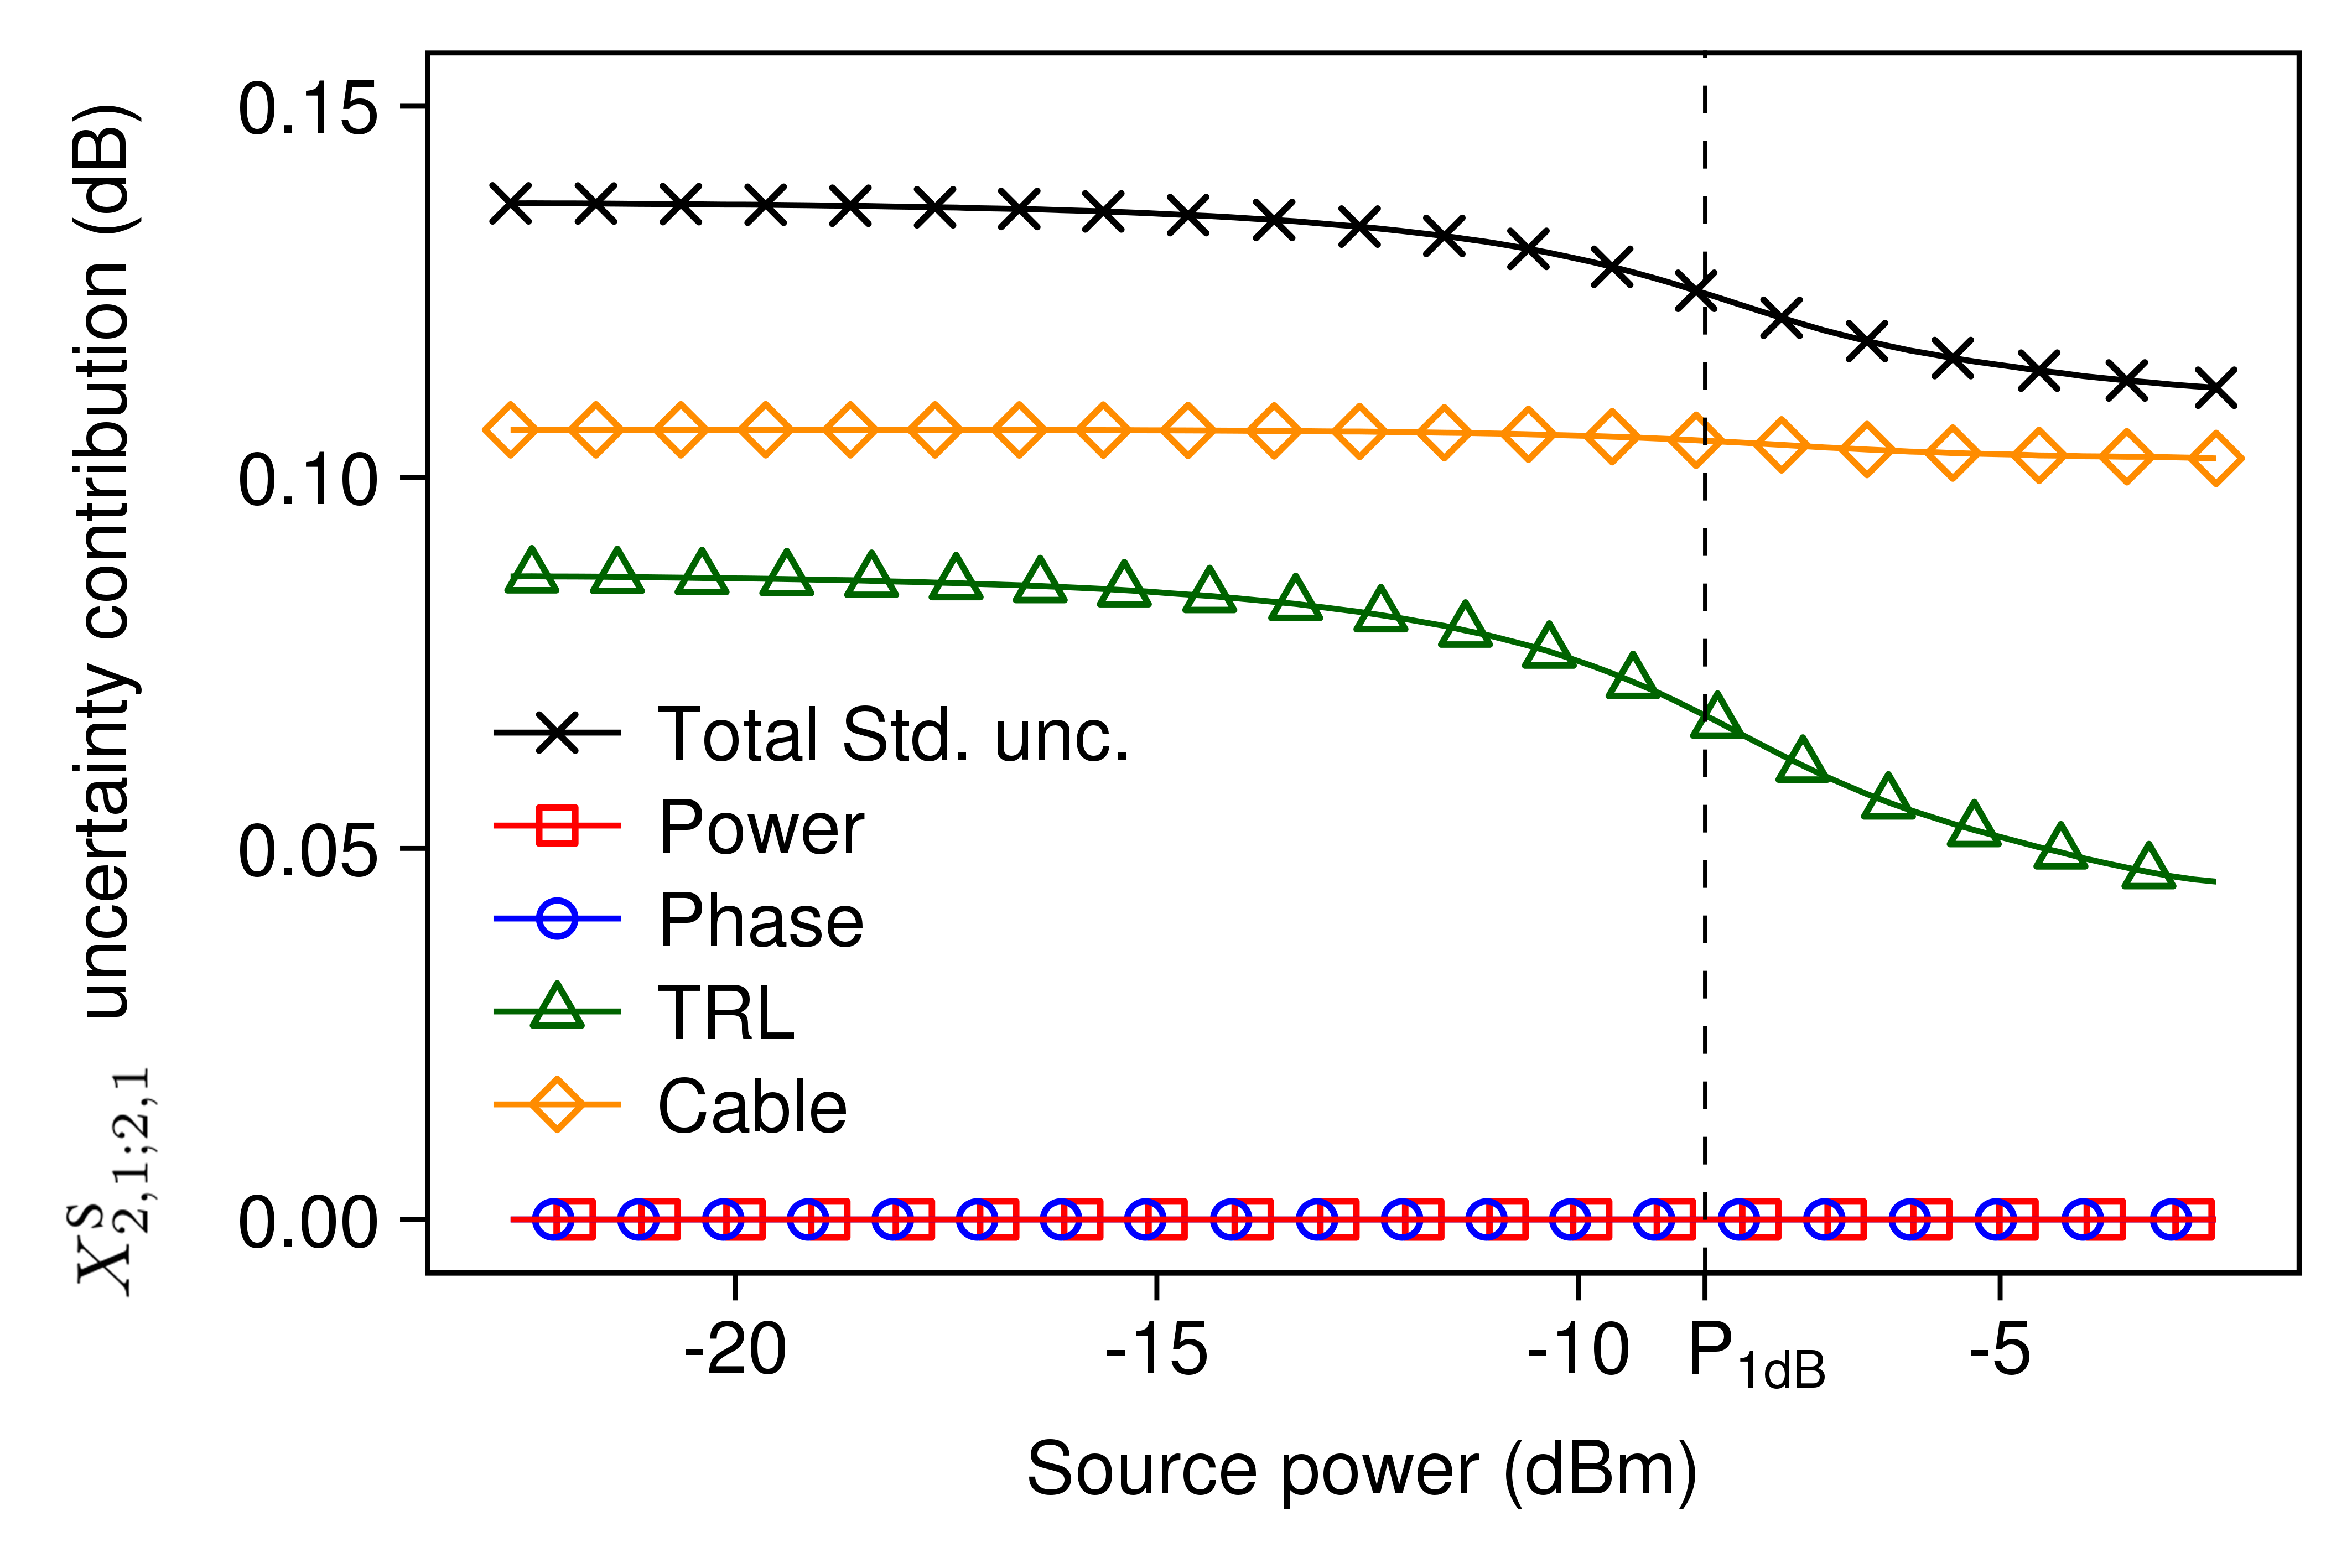
\includegraphics[width=\linewidth,height=5cm]{fig5c}
		\label{ch5_fig_s2121magsens}
	\end{subfigure}\hfil%
	\begin{subfigure}{0.45\textwidth}
		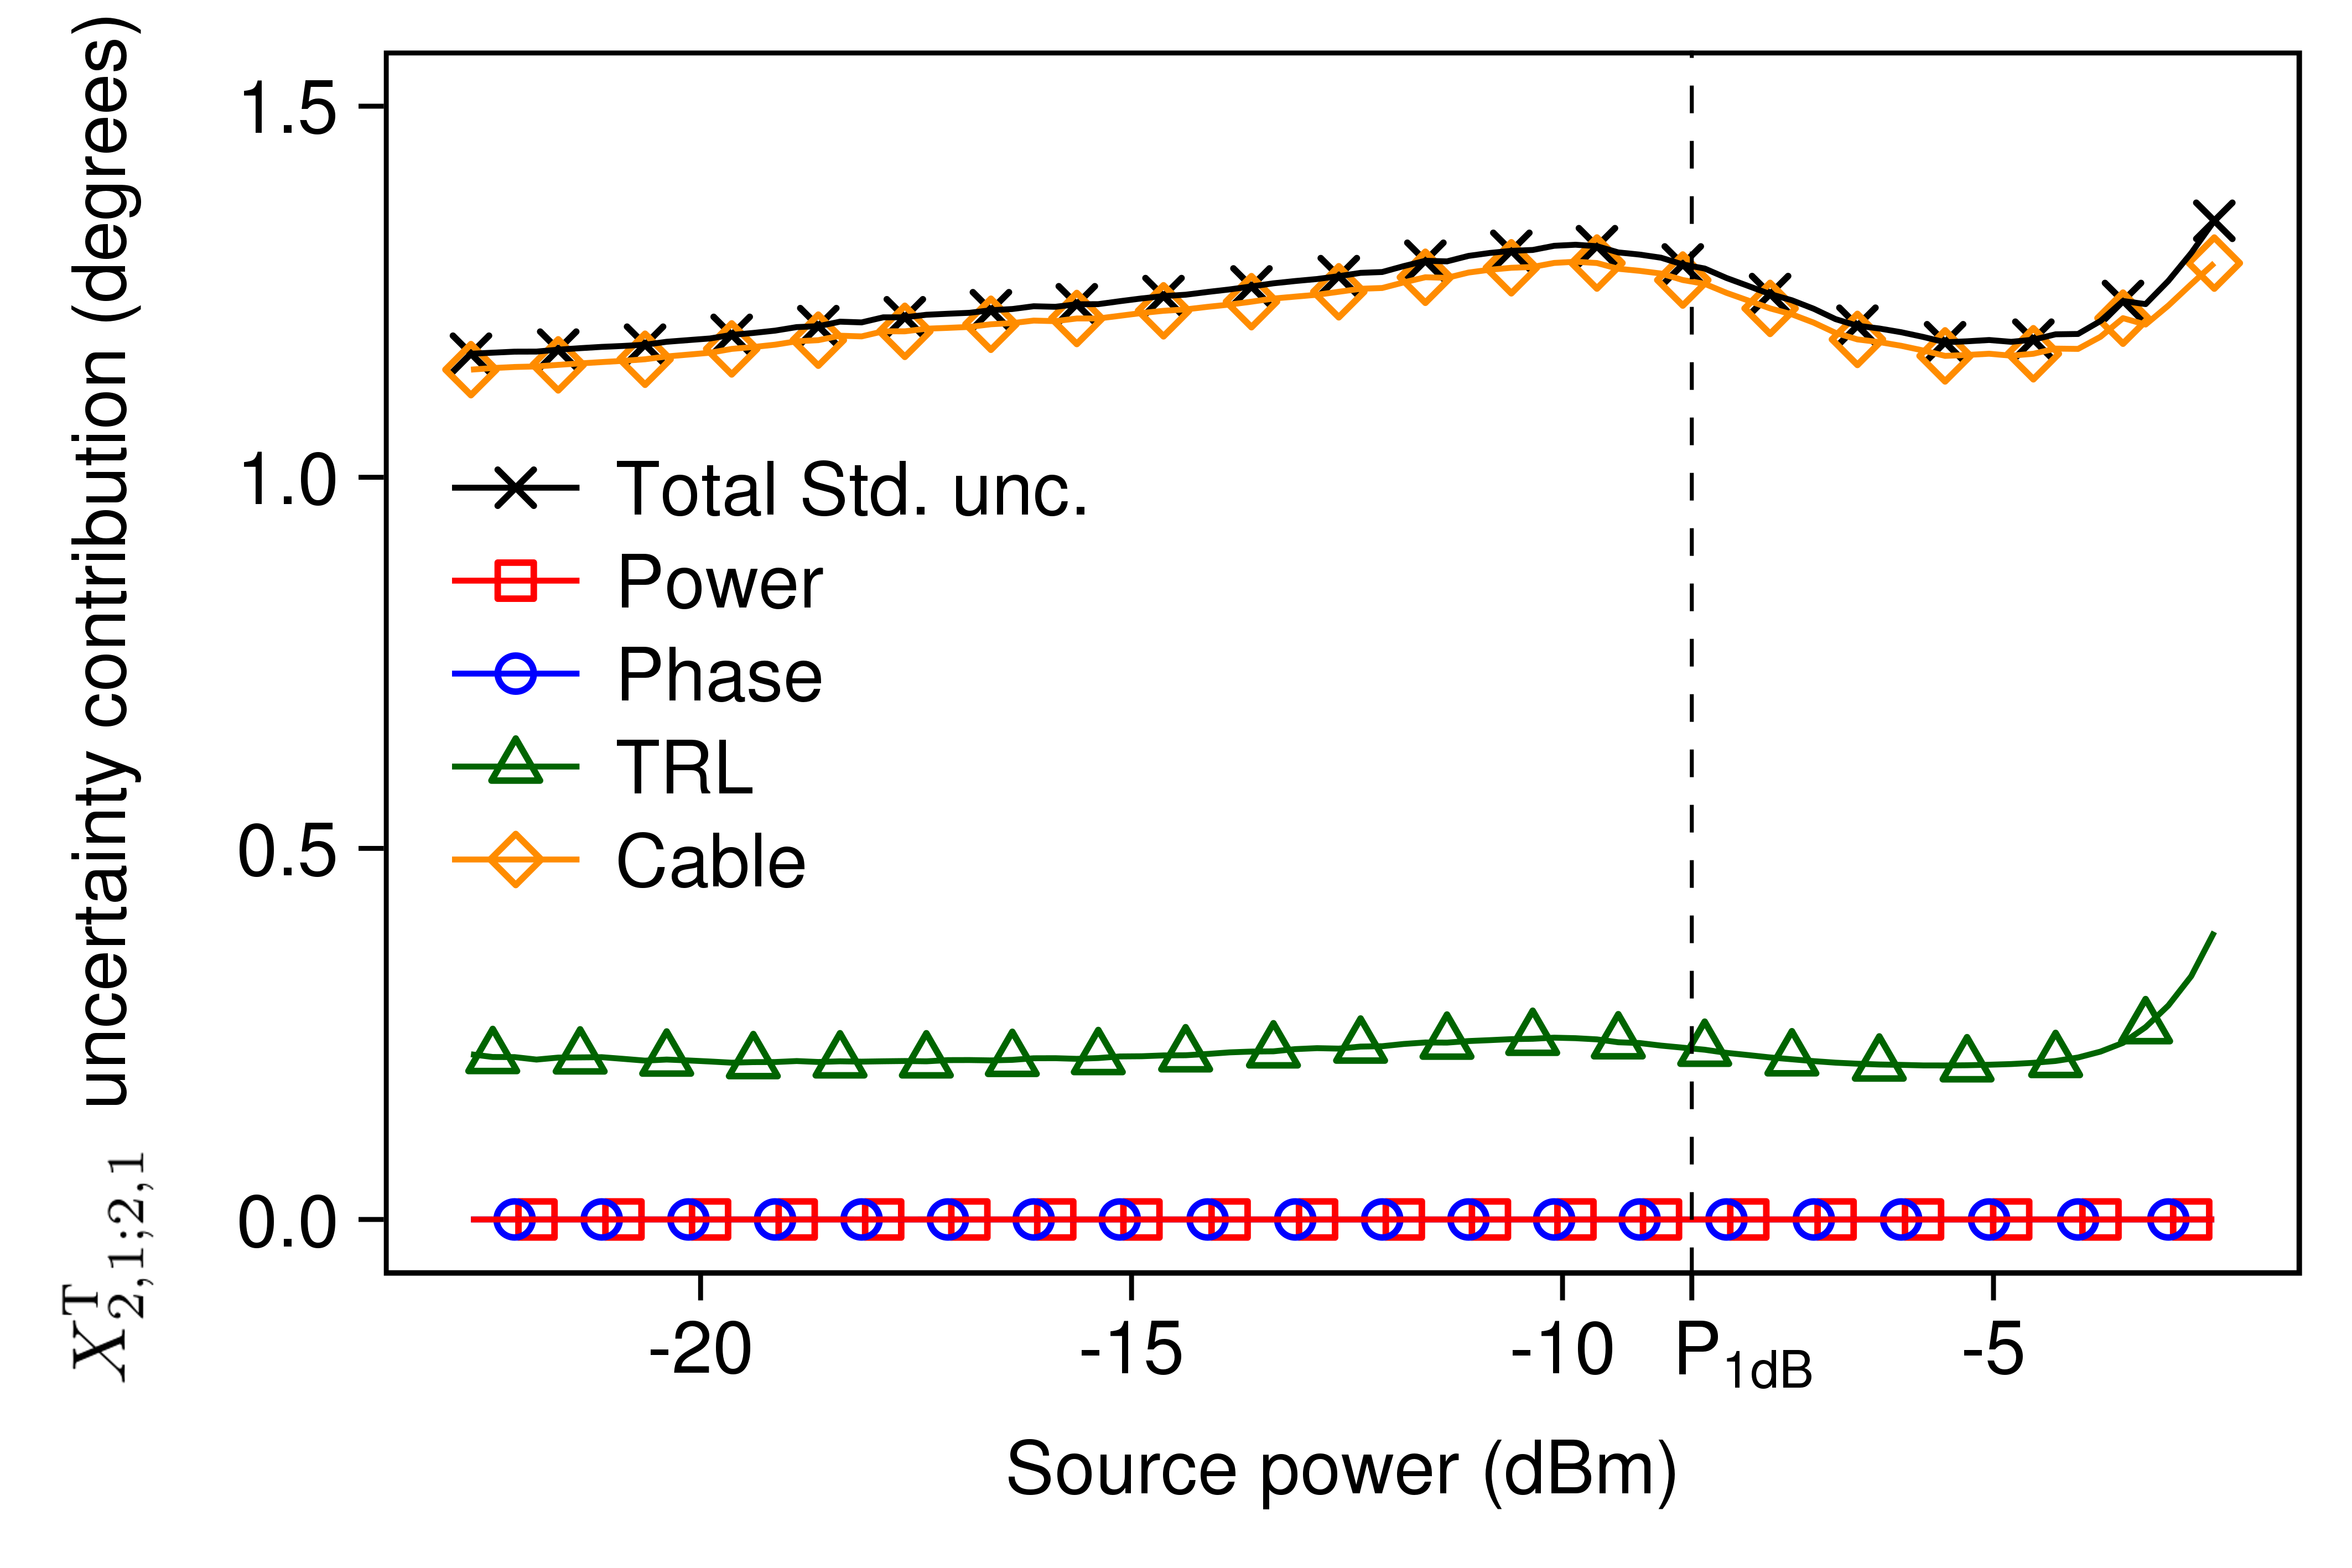
\includegraphics[width=\linewidth,height=5cm]{fig5d}	
		\label{ch5_fig_t2121phasesens}
	\end{subfigure}
	\caption{Sensitivity analysis results for a sample of the extracted X-parameters. Harmonic indices 1 and 2 relate to measurement frequencies of 25 and 50 GHz, respectively. Because the uncertainty is expressed as a linear variation of a decibel value, a non-zero horizontal line represents a linear relationship with source power.}
	\label{ch5_fig_sensplots}
\end{figure}

\section{Propagation of Uncertainty from X-Parameters into Circuit Simulations}

Once the behavioral model has been extracted from measurements, it can be used in circuit simulators to predict the performance of circuit designs. Because the uncertainty information is stored as a collection of samples, it can be propagated through the circuit simulator by sweeping the sample index and running the simulation for each value. From this array of results, a statistical analysis can be performed to determine the standard uncertainty of the performance metric in question. The sensitivity analysis can be propagated in a similar way, as there is a sample in the model file for the perturbation of each input quantity. It is also possible to evaluate uncertainty in circuit simulations containing multiple DUTs processed using the MUF, for example in a two-stage, balanced, or Doherty amplifier configuration. If the same variable is used to sweep the sample index for all DUTs, then any uncertainty correlations will be preserved. An example would be if multiple DUTs in the circuit were measured on an LSNA using the same calibration.
The measurement uncertainties which were captured into the X-parameter behavioral model can now be propagated to typical circuit metrics such as forward gain, input or output match, power-added efficiency (PAE), error vector magnitude (EVM) and adjacent channel power ratio (ACPR).

To demonstrate this, an example simulation has been created in Advanced Design System (ADS). The DUT is represented as an X-parameter model, and the simulator sweeps both the Monte Carlo sample index and the source power using the results from the MUF uncertainty evaluation. For this example the X-parameter file from the previous section was used. The schematic of the design is shown in Figure \ref{ch5_fig_schematic}, and typical design plots of gain and PAE are provided in Figure \ref{ch5_fig_adsplot}. It can be seen that although the uncertainties of both parameters increase significantly with source power, the 95\% expanded uncertainties are below 0.2 dB and 0.4\% for gain and PAE, respectively.

\begin{figure}
	\centering
	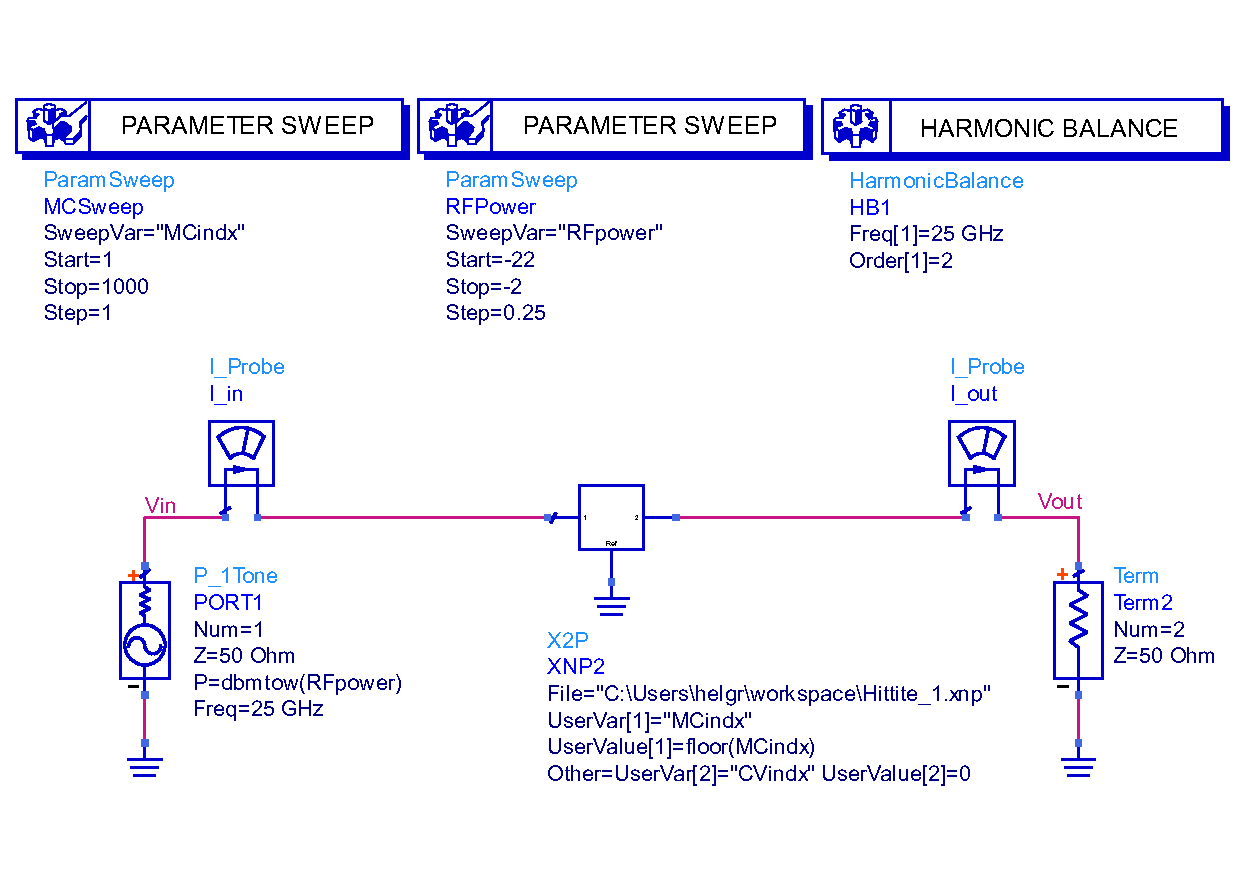
\includegraphics[width=0.8\textwidth]{fig6}
	\caption{An example circuit simulation schematic using an X-parameter model in ADS. The source power and X-parameter Monte Carlo sample index is swept by the Parameter Sweep components, and a harmonic balance simulation is carried out for each value of those sweeps.}
	\label{ch5_fig_schematic}
\end{figure}

\begin{figure}
	\centering
	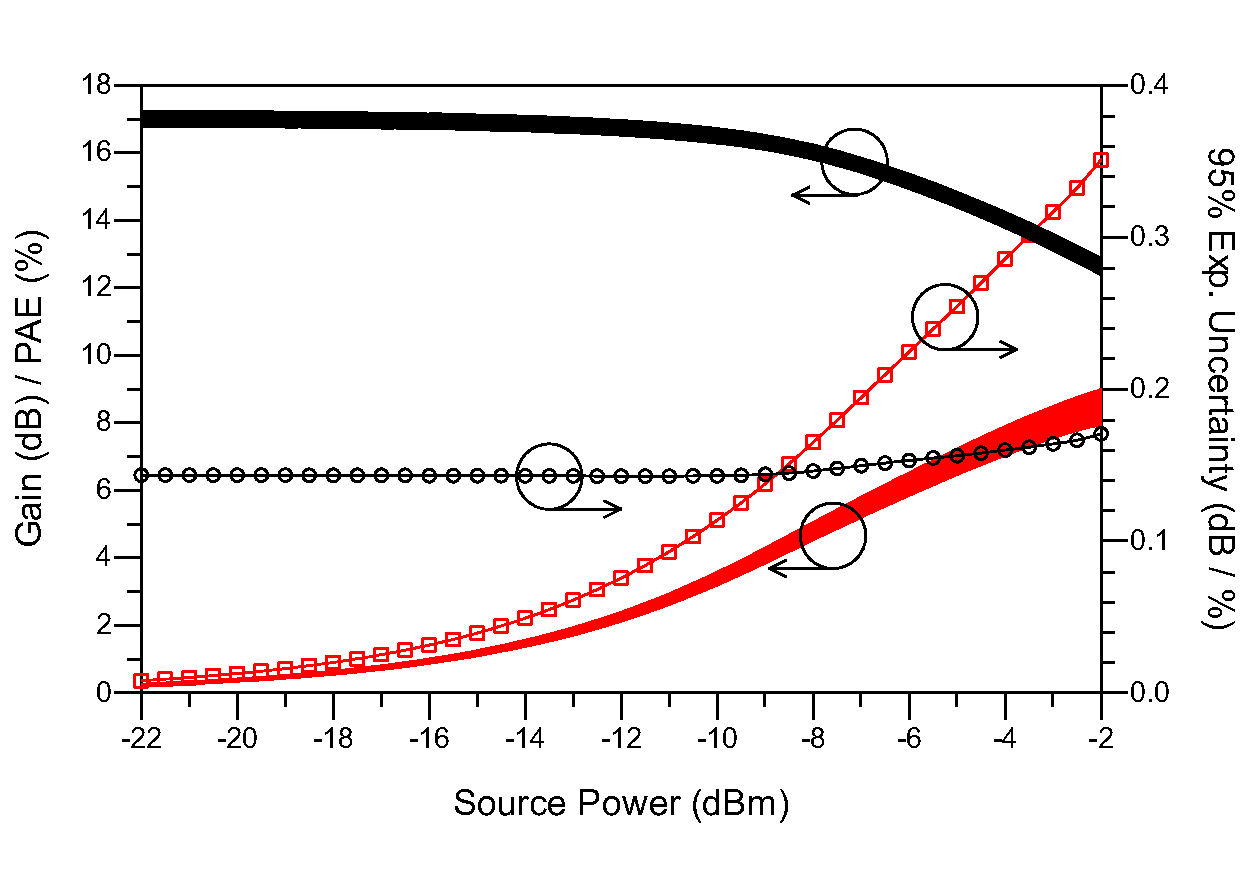
\includegraphics[width=0.8\textwidth]{fig7}
	\caption{Results from the ADS circuit simulation. The higher black trace shows the Monte Carlo samples for the gain of the circuit, whereas the lower red trace shows the PAE. The black trace with circles and red trace with squares show the 95\% expanded uncertainties for gain and PAE, respectively.}
	\label{ch5_fig_adsplot}
\end{figure}

\section{Conclusions}

This chapter has presented an overview of the main nonlinear behavioural models used to characterise microwave amplifiers for use in the design process. It is possible to see how over time the models have progressed from general but complicated Volterra and scattering function origins, through to more portable but simpler models such as X-parameters to promote industry usage, and finally the return to more capable solutions via the Cardiff model and X-parameter extensions.

A world-first, rigorous evaluation of combined standard uncertainty in nonlinear behaviour models of microwave and millimetre-wave amplifiers was presented, using a new framework based on the MUF through Monte Carlo and linear sensitivity analysis approaches. Both approaches preserve correlations between errors and provide a rigorous uncertainty evaluation. This has been demonstrated by extracting X-parameters with uncertainties from a typical millimeter-wave amplifier. The resulting model has been incorporated into circuit simulations to obtain gain and PAE results incorporating measurement uncertainty. The extracted amplifier model exhibited 95\% expanded uncertainties of less than 0.2 dB gain and less than 0.4\% PAE. 

To improve confidence in the design process of systems involving nonlinear devices, the uncertainty in both compact and behavioral models is required. This work has produced, for the first time, an evaluation of measurement uncertainty in a popular behavioral model, by developing a framework which can be easily adapted to support alternative models. In addition, the produced portable device model can be used in existing circuit simulators, allowing access to this information for statistical design techniques and to help achieve first pass design success for complicated nonlinear systems.

\addcontentsline{toc}{section}{Bibliography}
\printbibliography[title=References]
\end{refsection}
\end{document}
